%-----------------------------------------------------------------------------------------------------------%
\newpage

\part{پیشنیاز های ریاضی}
{
    \Large
    \begin{spacing}{1.4}
        \textbf{\vspace{3pt}}
        \begin{displayquote}
            راجر بیکن: زیرا چیزهای این جهان را نمی توان بدون دانش ریاضیات شناخت.
            \begin{flushleft}
                \lr{Opus Majus part 4 Distinctia Prima cap 1, 1267.}
            \end{flushleft}
        \end{displayquote}
        \textbf{\vspace{3pt}}

        بازی های ویدیویی سعی در شبیه سازی دنیای مجازی دارند.
        با این حال، کامپیوترها، به دلیل ماهیت خود، اعداد را محاسبه می کنند. بنابراین مشکل چگونگی انتقال جهان به کامپیوتر مطرح می شود.
        پاسخ این مشکل اینگونه است که جهان‌های ما و فعل و انفعالات موجود در آن را کاملاً ریاضی توصیف کنیم.
        در نتیجه، ریاضیات نقش اساسی در توسعه بازی های ویدیویی ایفا می کند.

        در این بخش، ابزارهای ریاضی که در این کتاب مورد استفاده قرار گرفته اند، معرفی می کنیم. تأکید ما بر بردارها، سیستم های مختصات، ماتریس ها و تبدیل ها است، زیرا این ابزارها تقریباً در همه ی برنامه های نمونه این کتاب استفاده شده اند.
        علاوه بر توضیحات ریاضی، بررسی و نمایش کلاس ها و توابع مربوطه از کتابخانه ریاضی \lr{DirectX} را نیز ارائه میکنیم.

        توجه داشته باشید که موضوعاتی که در اینجا مورد بررسی قرار می‌گیرند، تنها مواردی هستند که برای درک ادامه ی این کتاب ضروری اند.
        این کتاب به هیچ وجه راه حل جامعی برای ریاضیات بازی های ویدیویی نیست.

        \begin{point}{point:first}
            \Large
            برای خوانندگانی که مایل به ارجاع کامل تر به ریاضیات بازی های ویدیویی هستند، کتاب های زیر را توصیه می کنیم.
            \lr{
                \begin{enumerate}
                    \item {Essential Mathematics for Games and Interactive Applications: A Programmer's Guide (Verth04)}
                    \item {Mathematics for 3D Game Programming and Computer Graphics (Lengyel02)}
                \end{enumerate}
            }
            \textbf{\vspace{-20pt}}
        \end{point}

        \textbf{فصل 1، جبر برداری:} بردارها اساسی ترین اشیاء ریاضی مورد استفاده در بازی های کامپیوتری هستند.
        ما از بردارها برای نشان دادن موقعیت ها، جابجایی ها، جهت ها، سرعت ها و نیروها استفاده می کنیم.
        در این فصل، بردارها و عملیات مورد استفاده برای کار با آنها را مطالعه می کنیم.

        \textbf{فصل 2، جبر ماتریسی:} ماتریس ها روشی کارآمد و فشرده برای نمایش تبدیل ها ارائه می دهند.
        در این فصل با ماتریس ها و عملیات تعریف شده بر روی آنها آشنا می شویم.

        \textbf{فصل 3، تبدیل:} این فصل سه تبدیل هندسی اساسی را بررسی می کند: مقیاس بندی، چرخش و انتقال.
        ما از این تبدیل ها برای کار با اشیاء سه بعدی در فضا استفاده می کنیم.
        علاوه بر این، تغییر تبدیل مختصات را توضیح می دهیم، که برای تبدیل مختصات هندسی از یک سیستم مختصات به سیستم دیگر استفاده می شود.
    \end{spacing}
}

\setcounter{chapter}{1}

\textbf{\vspace{80pt}}


%\chapter{{\Large فصل 1}\Huge\\\textbf{\vspace{20pt}}1\textbf{جبر برداری}}
\chapter{\textbf{1 جبر برداری}}
\textbf{\vspace{70pt}}
{
    \Large
    \begin{spacing}{1.5}
        بردارها نقش مهمی در گرافیک کامپیوتری، تشخیص برخورد و شبیه سازی فیزیکی ایفا می کنند که همگی اجزای رایج در بازی های ویدئویی مدرن هستند.
        رویکرد ما در اینجا غیر تخصصی و عملی است به همین دلیل پیشنهاد ما کتاب \lr{Verth04} (نکته \ref{point:first}) است که کتابی اختصاصی برای ریاضیات بازی های سه بعدی/گرافیک است.
        ما بر اهمیت بردارها بسیار تأکید داریم زیرا در بیشتر برنامه های آزمایشی این کتاب استفاده شده اند.
        \\

        \textbf{\LARGE \hspace{-40pt}اهداف:}
        \begin{enumerate}
            \item {یادگیری نحوه نمایش بردارها به صورت هندسی و عددی}
            \item {یادگیری عملیات تعریف شده بر روی بردارها و کاربردهای هندسی آنها}
            \item {آشنایی با توابع برداری و کلاس های کتابخانه \lr{DirectXMath}}
        \end{enumerate}
    \end{spacing}
}
%-----------------------------------------------------------------------------------------------------------%
\newpage

\section{\textbf{بردار ها}}
{
    \Large
    \begin{spacing}{1.4}
        بردار به کمیتی اشاره دارد که هم اندازه و هم جهت دارد.
        به کمیت هایی که اندازه و جهت دارند، کمیت های برداری گویند.
        نمونه‌هایی از کمیت‌های برداری عبارتند از نیروها (نیرو در جهت خاصی با قدرت/اندازه معین اعمال می‌شود)، جابه‌جایی (جهت برآیند و فاصله حرکت ذره)، و سرعت‌ها (سرعت و جهت).
        بنابراین، بردارها برای نمایش نیروها، جابجایی ها و سرعت ها استفاده می شوند.
        به علاوه، ما از بردارها برای تعیین جهات خالص استفاده می کنیم،
        مانند جهتی که بازیکن در یک بازی سه بعدی به آن نگاه میکند،
        جهتی که یک چند ضلعی رو به آن قرار دارد، جهتی که پرتوی نور در آن حرکت می کند،
        یا جهتی که در آن یک پرتو نور از یک سطح منعکس می شود.

        اولین مرحله در توصیف ریاضی بردار ، توصیف هندسی آن است: ما به صورت گرافیکی یک بردار را با یک پاره خط جهت دار مشخص می کنیم (شکل \ref{fig:4.Session.1.1.1})، که در آن طول نشان دهنده بزرگی بردار و سر کمان نشان دهنده جهت بردار است.
        به این نکته باید توجه کنید که مکانی که در آن یک بردار رسم می‌کنیم بی‌اهمیت است، زیرا تغییر مکان، بزرگی یا جهت را تغییر نمی‌دهد (دو ویژگی ای که بردار دارد).
        بنابراین می گوییم دو بردار برابر هستند اگر و تنها اگر طول یکسانی داشته و در یک جهت باشند.
        بنابراین، بردارهای \lr{u} و \lr{v} ترسیم شده در قسمت آ شکل \ref{fig:4.Session.1.1.1} در واقع برابر اند زیرا طول و جهت یکسانی دارند.
        در واقع، چون مکان برای بردارها اهمیتی ندارد، ما می‌توانیم یک بردار را بدون تغییر هویت آن ، انتقال دهیم (زیرا انتقال نه طول و نه جهت را تغییر می‌دهد).
        توجه داشته باشید که ما می‌توانیم \lr{u} را طوری انتقال دهیم که کاملاً بر \lr{v} همپوشانی داشته باشد (و بالعکس) و در نتیجه آنها را غیرقابل تشخیص کنیم. این نیز دلیلی برای برابری آنهاست.

        \begin{figure}[H]
            \centering
            \setlength{\belowcaptionskip}{-10pt}
            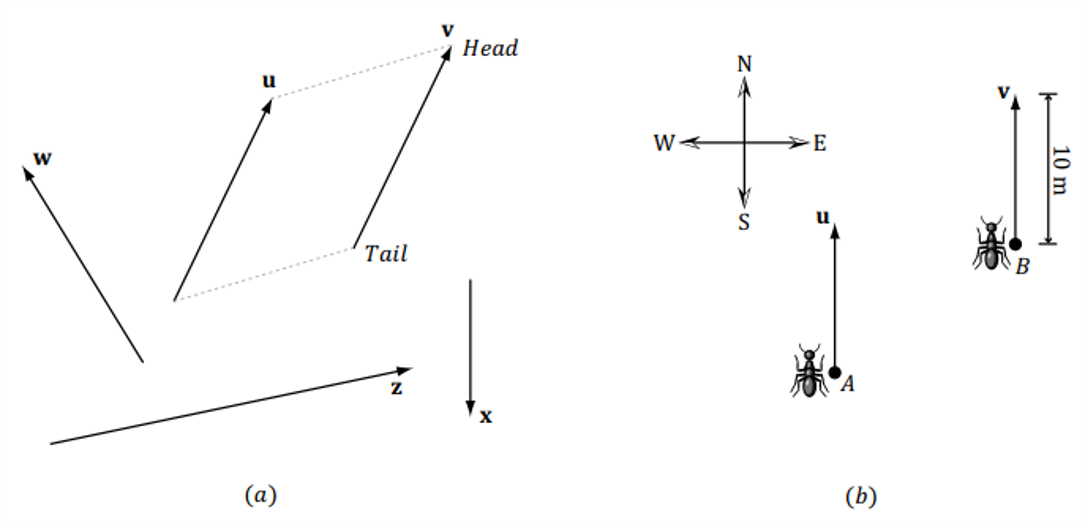
\includegraphics[width=0.85\textwidth]{Images/4/4.Session.1.1.1}
            \caption{(الف) بردار هایی که روی صفحه ی دوبعدی کشیده شده اند.
                (ب) بردار هایی که مورچه ها را برای حرکت 10 متر در جهت شمال راهنمایی میکنند.}
            \label{fig:4.Session.1.1.1}
        \end{figure}

        به عنوان یک مثال فیزیکی، بردارهای \lr{u} و \lr{v} در قسمت ب شکل \ref{fig:4.Session.1.1.1} هر دو به مورچه ها میگویند در دو نقطه مختلف \lr{A} و \lr{B} ده متر به سمت شمال حرکت کنند.
        دوباره \lr{u = v} را داریم.
        بردارها خود مستقل از موقعیت هستند و
        آنها به سادگی به مورچه ها آموزش می دهند که چگونه از جایی که هستند، ده متر (طول) به سمت شمال (جهت) حرکت کنند.

    \end{spacing}
}

\subsection{\textbf{بردارها و سیستم های مختصات}}
{
    \Large
    \begin{spacing}{1.5}
        اکنون می‌توانیم عملیات هندسی مفیدی را روی بردارها تعریف کنیم، که سپس می‌توان از آنها برای حل مسائل مربوط به کمیت‌های برداری استفاده کرد.
        با این حال، از آنجایی که کامپیوتر نمی تواند با بردارها به صورت هندسی کار کند، باید راهی برای تعیین عددی بردارها پیدا کنیم.
        بنابراین یک سیستم مختصات سه بعدی را در فضا معرفی می کنیم و همه بردارها را طوری انتقال میدهیم که دم آن ها با مبدا منطبق باشد (شکل \ref{fig:4.Session.1.1.2}).

        \begin{figure}[H]
            \centering
            \setlength{\belowcaptionskip}{-10pt}
            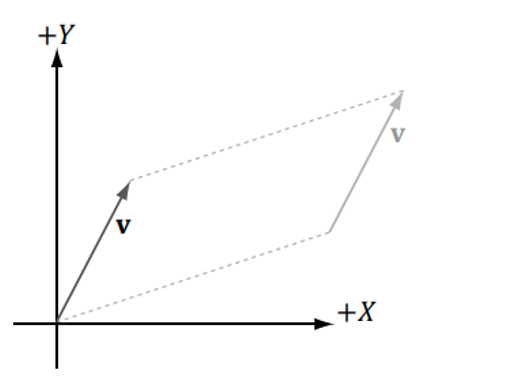
\includegraphics[width=0.48\textwidth]{Images/4/4.Session.1.1.2}
            \caption{\lr{v} را طوری انتقال میدهیم که دم آن با مبدأ سیستم مختصات منطبق
            باشد. وقتی دم یک بردار با مبدا منطبق می شود، می گوییم که در موقعیت استاندارد قرار دارد.}
            \label{fig:4.Session.1.1.2}
        \end{figure}

        سپس می‌توانیم یک بردار را با تعیین مختصات سر آن شناسایی کنیم و مانند شکل \ref{fig:4.Session.1.1.3}، \lr{v = (x, y, z)} را بنویسیم.
        اکنون می توانیم یک بردار را با سه \lr{float} در یک برنامه کامپیوتری نشان دهیم.

        \begin{point}{pnt:2}
            \Large
            اگر کار به صورت \lr{2D} باشد، فقط از یک سیستم مختصات \lr{2D} استفاده می کنیم و بردار فقط دو مختصات دارد:
            \lr{v = (x, y)} و یک بردار را با دو \lr{float} در یک برنامه نشان میدهیم.
        \end{point}

        \begin{figure}[H]
            \centering
            \setlength{\belowcaptionskip}{-10pt}
            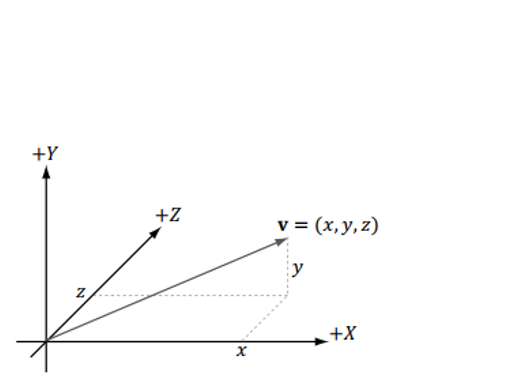
\includegraphics[width=0.48\textwidth]{Images/4/4.Session.1.1.3}
            \caption{یک بردار مشخص شده توسط مختصات نسبت به یک سیستم مختصات.}
            \label{fig:4.Session.1.1.3}
        \end{figure}

        شکل \ref{fig:4.Session.1.1.4} را در نظر بگیرید که یک بردار \lr{v} و دو فریم (\lr{frame}) در فضا را نشان می دهد. (توجه داشته باشید که ما از اصطلاحات فریم، فریم مرجع، فضا و سیستم مختصات استفاده می کنیم که همگی در این کتاب به یک معنا هستند.)
        می توانیم \lr{v} را طوری انتقال دهیم که در هر یک از دو سیستم مختصات در موقعیت استاندارد قرار گیرد. با این حال، مشاهده کنید که مختصات بردار \lr{v} نسبت به سیستم مختصات \lr{A} با مختصات بردار \lr{v} نسبت به سیستم مختصات \lr{B} متفاوت است.
        به عبارت دیگر، همان بردار \lr{v} نمایش مختصاتی متفاوتی برای سیستم مختصات های متمایز دارد.

        \begin{figure}[H]
            \centering
            \setlength{\belowcaptionskip}{-10pt}
            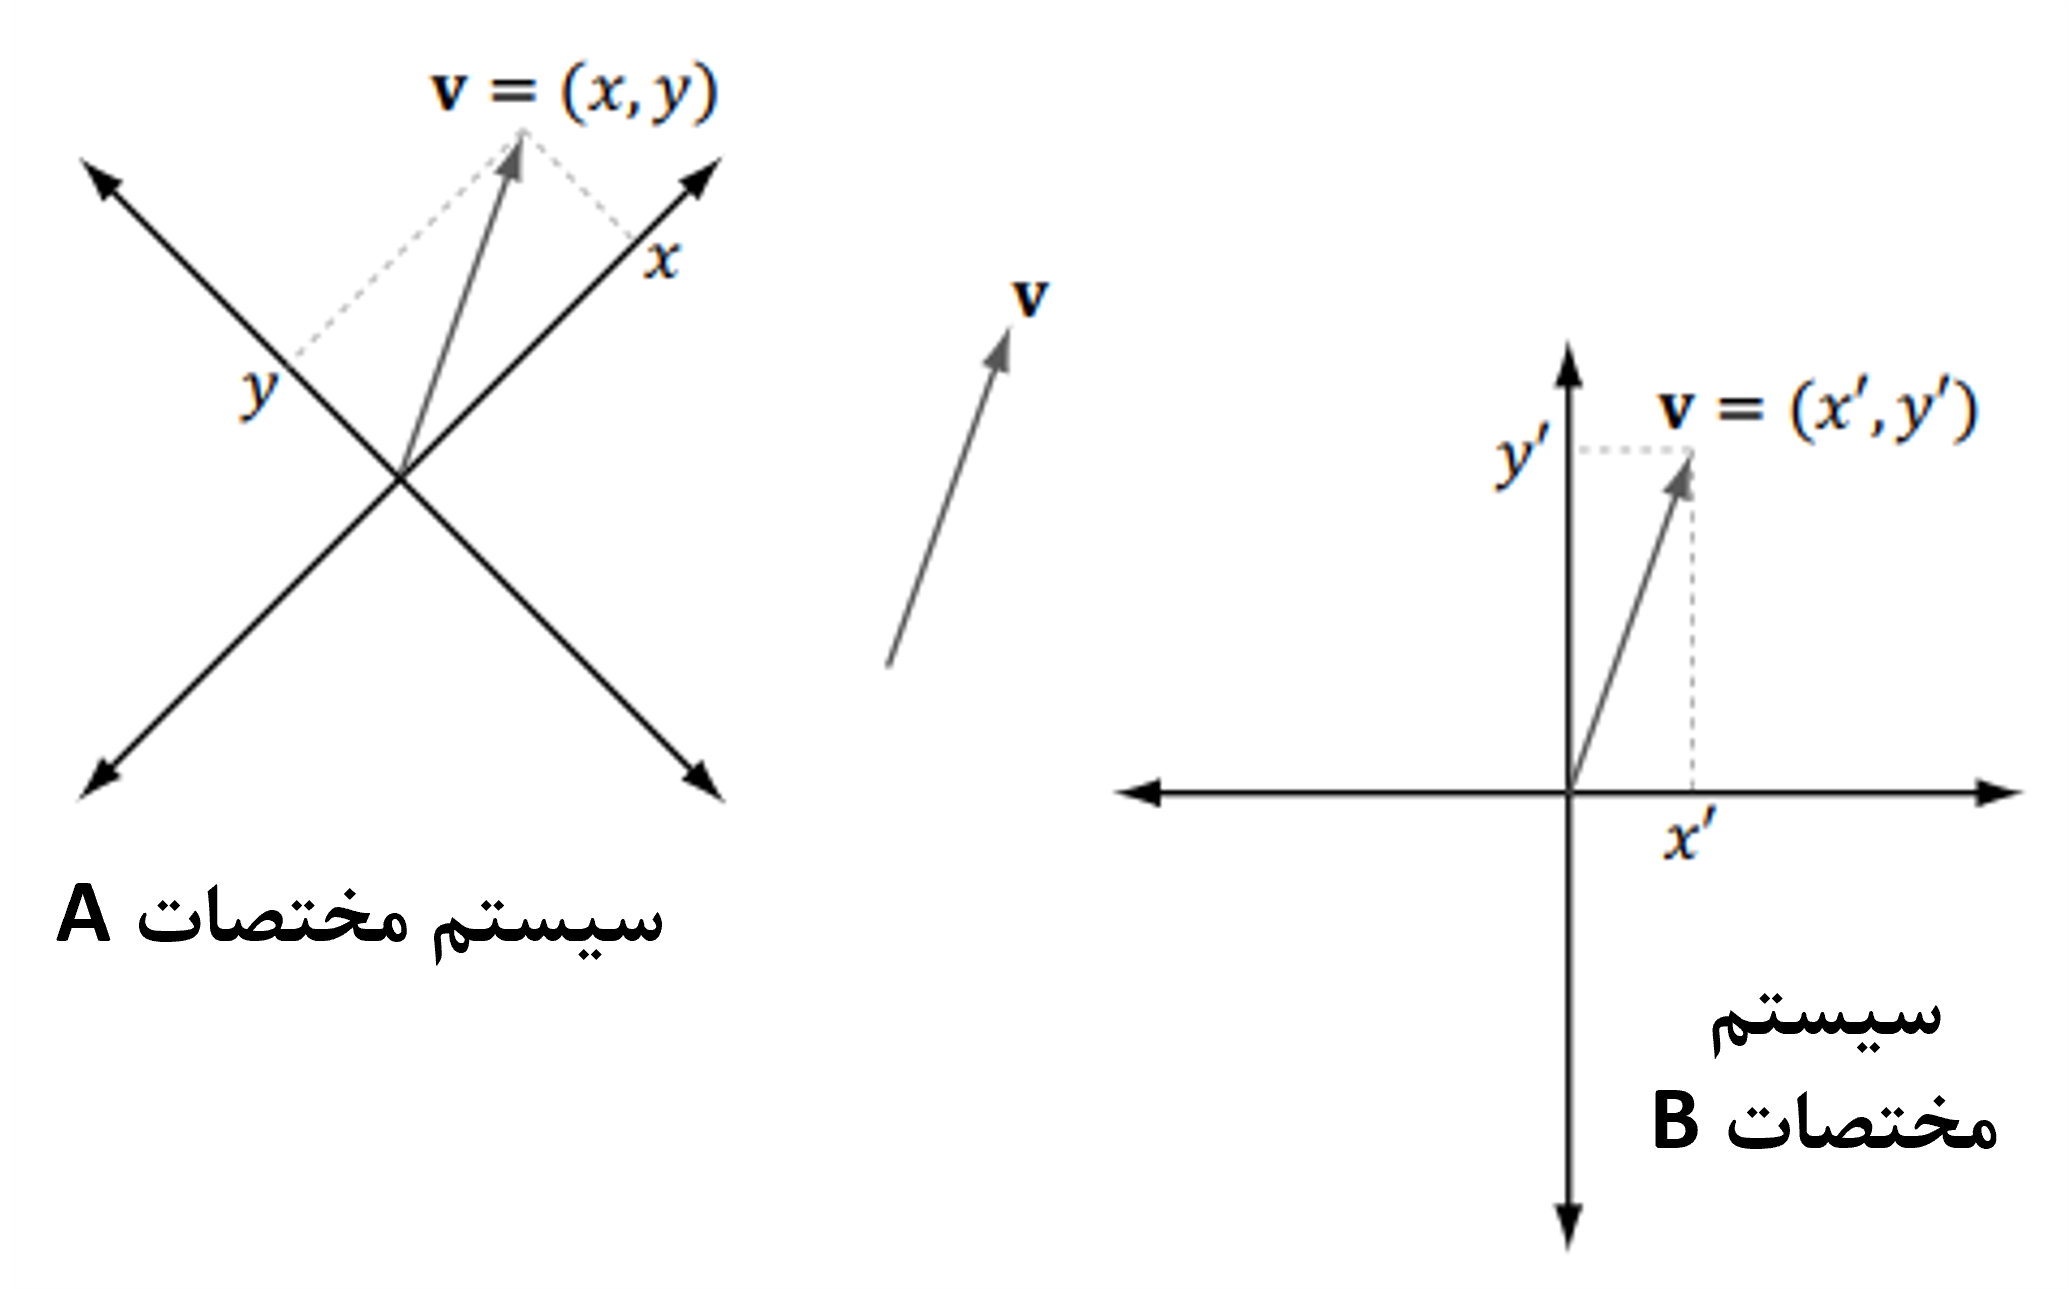
\includegraphics[width=0.8\textwidth]{Images/4/4.Session.1.1.4}
            \caption{همان بردار v زمانی که نسبت به سیستم مختصات های مختلف تعریف شود، مختصات متفاوتی دارد.}
            \label{fig:4.Session.1.1.4}
        \end{figure}

        این ایده شبیه به مثال دما است. آب در 100 درجه سانتیگراد یا 212 درجه فارنهایت می جوشد.
        دمای فیزیکی آب جوش بدون توجه به مقیاس یکسان است (یعنی نمی‌توانیم نقطه جوش را با انتخاب مقیاس متفاوت کاهش دهیم)،
        اما بر اساس مقیاسی که استفاده می‌کنیم عدد اسکالر متفاوتی را به دما اختصاص می‌دهیم.
        به طور مشابه، برای یک بردار، جهت و بزرگی آن، که در پاره خط جهت دار تعبیه شده است، تغییر نمی کند.
        فقط مختصات آن بر اساس سیستم مختصات که برای توصیف آن استفاده می کنیم تغییر می کند.
        این نکته ی مهمی ست زیرا به این معنی است که هرگاه یک بردار را با مختصات شناسایی کنیم، آن مختصات نسبت به برخی از سیستم های مختصات هستند.
        اغلب در گرافیک های کامپیوتری سه بعدی، از بیش از یک سیستم مختصات استفاده می کنیم و بنابراین، باید شناسایی کنیم که مختصات یک بردار نسبت به کدام سیستم مختصات است.
        علاوه بر این، ما باید بدانیم که چگونه مختصات برداری را از یک سیستم مختصات به سیستم مختصات دیگر تبدیل کنیم.
        \textbf{\vspace{-10pt}}
        \begin{point}{pnt:3}
            \Large
            مشاهده میکنیم که بردارها و نقاط را می توان با مختصات (\lr{x, y, z}) نسبت به یک سیستم مختصات توصیف کرد.
            با این حال، بردارها و نقاط یکسان نیستند؛ یک نقطه نشان دهنده یک مکان در 3 فاصله است، در حالی که یک بردار نشان دهنده یک اندازه و جهت است.
        \end{point}
        \textbf{\vspace{-50pt}}
    \end{spacing}

    \begin{figure}[H]
        \centering
        \setlength{\belowcaptionskip}{-10pt}
        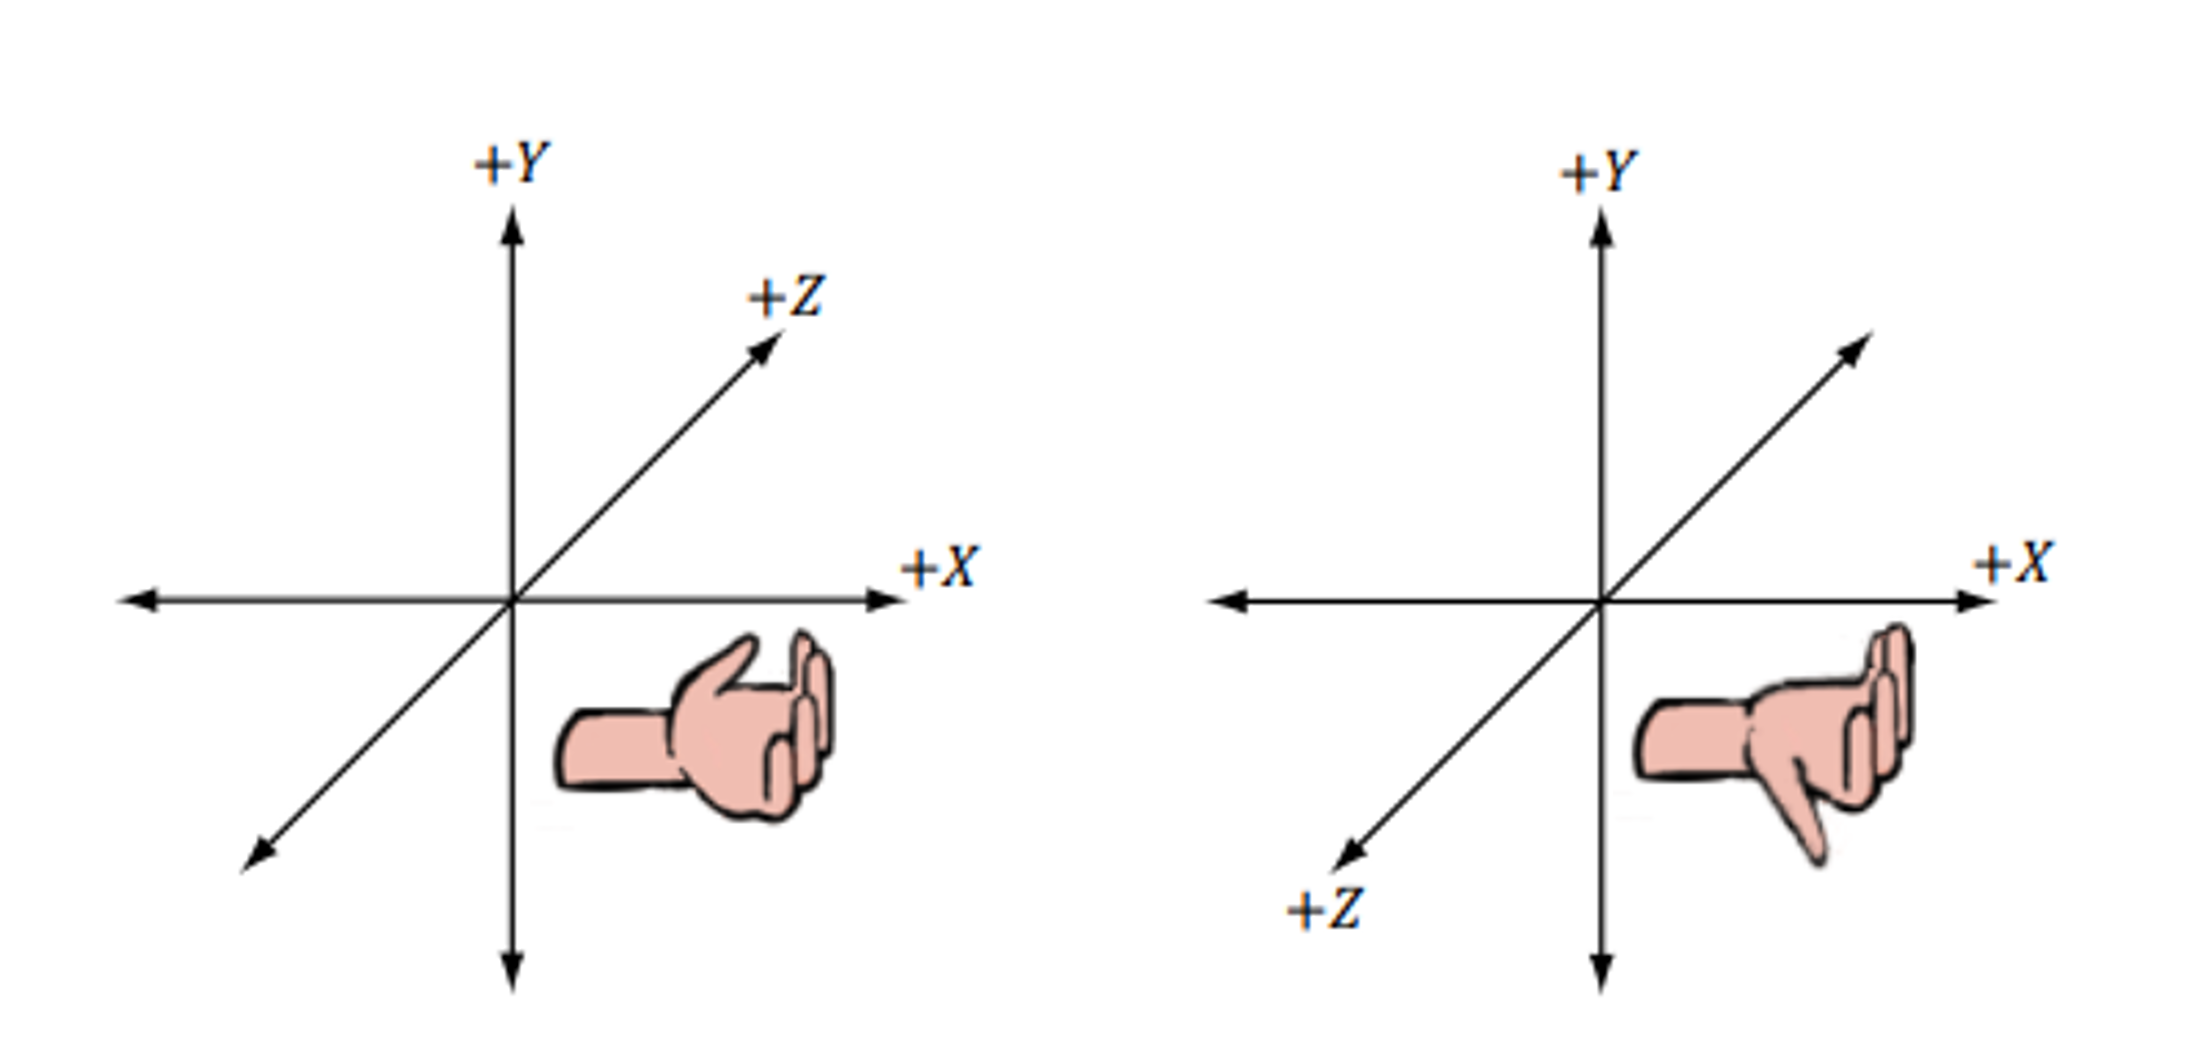
\includegraphics[width=0.9\textwidth]{Images/4/4.Session.1.1.5}
        \caption{در سمت چپ ما یک سیستم مختصات چپگرد داریم که محور z مثبت وارد صفحه می شود. در سمت راست ما یک سیستم مختصات راستگرد داریم که محور z مثبت از صفحه خارج می شود.}
        \label{fig:4.Session.1.1.5}
    \end{figure}
}

\subsection{\textbf{سیستم های مختصات چپگرد در مقابل راستگرد}}
{
    \Large
    \begin{spacing}{1.5}
        \lr{Direct3D} از یک سیستم مختصات چپگرد استفاده می کند.
        اگر دست چپ خود را به صورتی بگیرید که انگشتان خود را به سمت محور x مثبت گرفته و سپس انگشتان خود را به سمت محور y مثبت خم کنید، انگشت شست شما در جهت محور z مثبت قرار می گیرد.
        شکل \ref{fig:4.Session.1.1.5} تفاوت بین یک سیستم مختصات چپ دست و راست دست را نشان می دهد.
        توجه کنید که در سیستم مختصات راستگرد، اگر دست راست خود را به صورتی بگیرید که انگشتان خود را به سمت محور x مثبت گرفته و سپس انگشتان خود را به سمت محور y مثبت خم کنید، انگشت شست شما در جهت محور z مثبت اشاره می کند.

    \end{spacing}
}

\subsection{\textbf{عملیات بردار پایه}}
{
    \Large
    \begin{spacing}{1.5}
        اکنون با استفاده از نمایش مختصاتی، تساوی، جمع، ضرب اسکالر و تفریق را بر روی بردارها تعریف می کنیم.
        برای این چهار تعریف، فرض میکنیم $\textbf{u}=(u_{x},u_{y},u_{z})$ و  $\textbf{v}=(v_{x},v_{y},v_{z})$.

        \begin{enumerate}
            \item {دو بردار مساوی هستند اگر و تنها اگر اجزای متناظر آنها با هم برابر باشند.
            یعنی $\textbf{u}=\textbf{v}$ اگر و تنها اگر $u_{x}=v_{x}$ ، $u_{y}=v_{y}$ و $u_{z}=v_{z}$}
            \item {بردارها را به صورت جزء اضافه می کنیم: $\textbf{u}+\textbf{v}=(u_{x}+v_{x},u_{y}+v_{y},u_{z}+v_{z})$.
            توجه داشته باشید که فقط اضافه کردن بردارهایی با همان بعد ، منطقی ست.}
            \item {می توانیم یک اسکالر (یعنی یک عدد حقیقی) و یک بردار را ضرب کنیم و نتیجه یک بردار خواهد بود.
            فرض کنید k یک اسکالر باشد، پس $k\textbf{u}=(ku_{x},ku_{y},ku_{z})$. به این ضرب اسکالر می گویند.}
            \item {ما تفریق را بر حسب جمع بردار و ضرب اسکالر انجام می دهیم.
            یعنی $\textbf{u}-\textbf{v}=\textbf{u}+(-1\cdot\textbf{v})=\textbf{u}+(-\textbf{v})=(u_{x}-v_{x},u_{y}-v_{y},u_{z}-v_{z})$}
        \end{enumerate}

        \textbf{\vspace{-6pt}}
        \begin{example}{exp:1}
            \Large
            فرض کنید $\textbf{u}=(1,2,3), \textbf{v}=(1,2,3), \textbf{w}=(3,0,-2), k=2$
            \lr{
                \begin{enumerate}
                    \item {$\textbf{u}+\textbf{w}=(1,2,3)+(3,0,-2)=(4,2,1)$}
                    \item {$\textbf{u}=\textbf{v}$}
                    \item {$\textbf{u}-\textbf{v}=\textbf{u}+(-\textbf{v})=(1,2,3)+(-1,-2,-3)=(0,0,0)=\textbf{0}$}
                    \item {$k\textbf{w}=2(3,0,-2)=(6,0,-4)$}
                \end{enumerate}
            }
            تفاوتی که در مورد سوم هست ، یک بردار خاص به نام بردار صفر را نشان می دهد که همه اجزای آن صفر است و با \lr{\textbf{0}} نشان داده می شود.
        \end{example}

        \textbf{\vspace{-6pt}}
        \begin{example}{exp:2}
            \Large
            ما این مثال را با بردارهای دوبعدی برای ساده‌تر کردن کار توضیح می‌دهیم. ایده ها مانند فضای سه بعدی هستند، فقط با یک جزء کمتر ، به صورت دو بعدی کار می کنیم.\\
            \begin{enumerate}
                \item {فرض کنید $\textbf{v}=(2,1)$، $\textbf{v}$ و $-\frac{\displaystyle 1}{\displaystyle 2}\textbf{v}$ چگونه از نظر هندسی با هم مقایسه می شوند؟
                توجه داریم که $-\frac{\displaystyle 1}{\displaystyle 2}\textbf{v}=(-1,-\frac{\displaystyle 1}{\displaystyle 2})$.
                با ترسیم نمودار $\textbf{v}$ و $-\frac{\displaystyle 1}{\displaystyle 2}\textbf{v}$ (قسمت آ شکل \ref{fig:4.Session.1.1.6})،
                متوجه می‌شویم که $-\frac{\displaystyle 1}{\displaystyle 2}\textbf{v}$ در جهت مخالف $\textbf{v}$ است و طول آن $\frac{\displaystyle 1}{\displaystyle 2}\textbf{v}$ است.
                بنابراین، از نظر هندسی، منفی کردن یک بردار را می‌توان به صورت "برگرداندن" جهت آن،
                و ضرب اسکالر را می توان به عنوان مقیاس بندی طول یک بردار در نظر گرفت.}\\

                \item {فرض کنید $\textbf{u}=(2,\frac{\displaystyle 1}{\displaystyle 2})$ و $\textbf{v}=(1,2)$. پس $\textbf{u}+\textbf{v}=(3,\frac{\displaystyle 5}{\displaystyle 2})$ .
                قسمت ب شکل \ref{fig:4.Session.1.1.6} نشان می‌دهد که جمع بردار از نظر هندسی به چه معناست:
                ما $\textbf{u}$ را به‌طور موازی انتقال میدهیم تا دم آن با سر $\textbf{v}$ منطبق شود.
                پس بردار مجموع ، برداری است که از دم $\textbf{v}$ شروع شده و با سر $\textbf{u}$ منتقل شده ختم می‌شود.
                    (اگر $\textbf{u}$ را ثابت نگه داریم و $\textbf{v}$ را طوری انتقال دهیم که دم آن با سر $\textbf{u}$ منطبق شود، همین نتیجه را می گیریم.
                    در این حالت، $\textbf{u}+\textbf{v}$ برداری خواهد بود که از دم $\textbf{u}$ شروع شده و با سر $\textbf{v}$ منتقل شده ختم میشود.)
                    توجه داشته باشید که قوانین جمع بردار در زمانی که نیروها را با هم جمع می کنیم تا نیروی برآیند را به وجود بیاوریم، با انتظار ما مطابقت دارد:
                    اگر دو نیرو (بردار) را در یک راستا اضافه کنیم، نیروی برآیند قوی تری (بردار طولانی تر) در آن جهت دریافت می کنیم.
                    اگر دو نیرو (بردار) مخالف یکدیگر را بهم اضافه کنیم، نیروی برآیند ضعیف تری (بردار کوتاه تر) به دست می آید.
                    شکل \ref{fig:4.Session.1.1.7} این ایده ها را نشان می دهد.}\\

                \item {فرض کنید $\textbf{v}=(2,1)$، $\textbf{v}$ و $\textbf{v}-\textbf{u}=(-1,\frac{\displaystyle 3}{\displaystyle 2})$. پس
                قسمت پ شکل \ref{fig:4.Session.1.1.6} نشان می دهد که تفریق برداری از نظر هندسی به چه معناست.
                    $\textbf{v}-\textbf{u}$ به ما یک بردار با از سر $\textbf{u}$ تا سر $\textbf{v}$ می دهد.
                    اگر در عوض u و v را به عنوان نقاط تفسیر کنیم، آنگاه $\textbf{v}-\textbf{u}$ برداری را با هدف از نقطه $\textbf{u}$ تا نقطه $\textbf{v}$ به ما می دهد.
                    این تفسیر مهم است زیرا ما اغلب می خواهیم که بردار از یک نقطه به نقطه دیگر برود.
                    همچنین طول $\textbf{v}-\textbf{u}$ فاصله $\textbf{u}$ تا $\textbf{v}$ است، وقتی که $\textbf{u}$ و $\textbf{v}$ را به عنوان نقطه در نظر بگیریم.}
            \end{enumerate}

            \begin{figure}[H]
                \centering
                \setlength{\belowcaptionskip}{-10pt}
                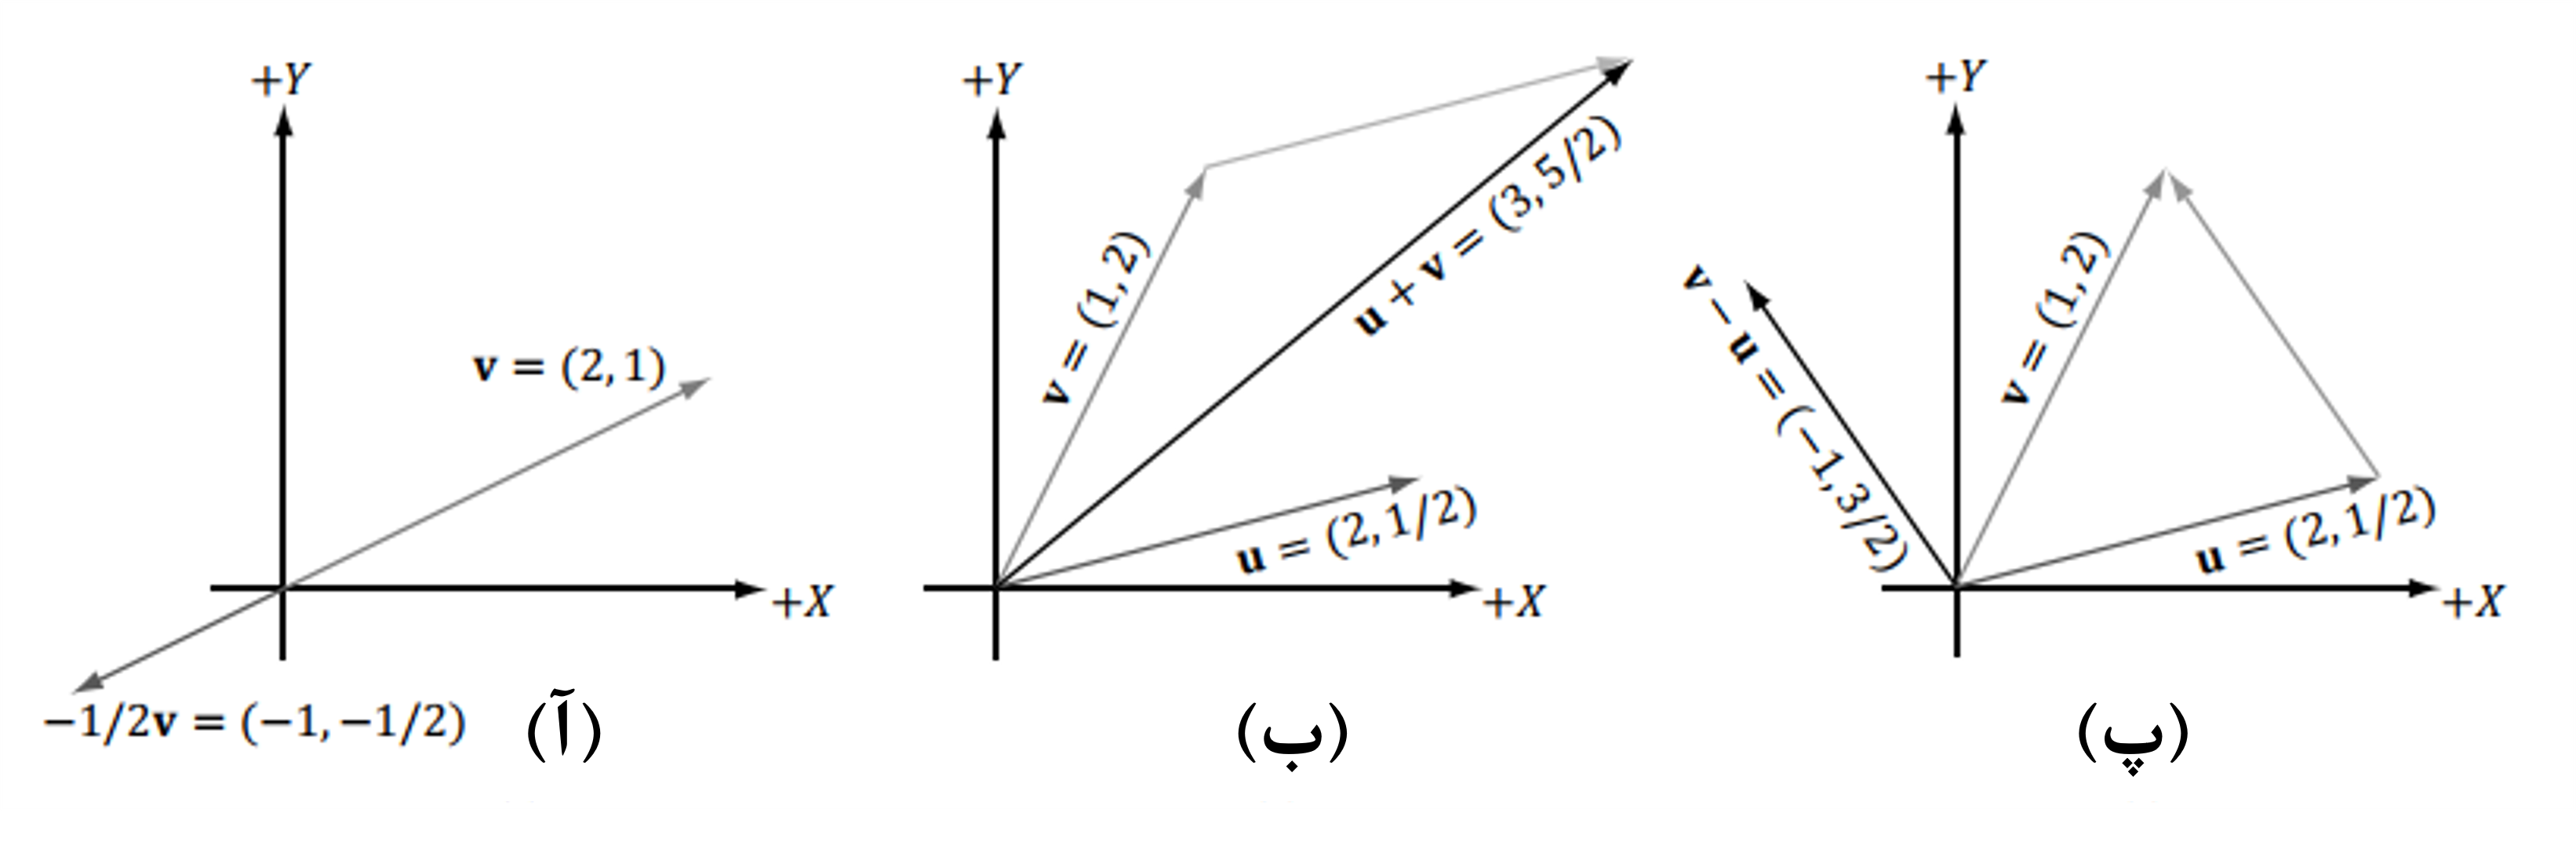
\includegraphics[width=\textwidth]{Images/4/4.Session.1.1.6}
                \caption{(آ) تفسیر هندسی ضرب اسکالر. (ب) تفسیر هندسی جمع بردار. ج) تفسیر هندسی تفریق بردار.}
                \label{fig:4.Session.1.1.6}
            \end{figure}

            \begin{figure}[H]
                \centering
                \setlength{\belowcaptionskip}{-10pt}
                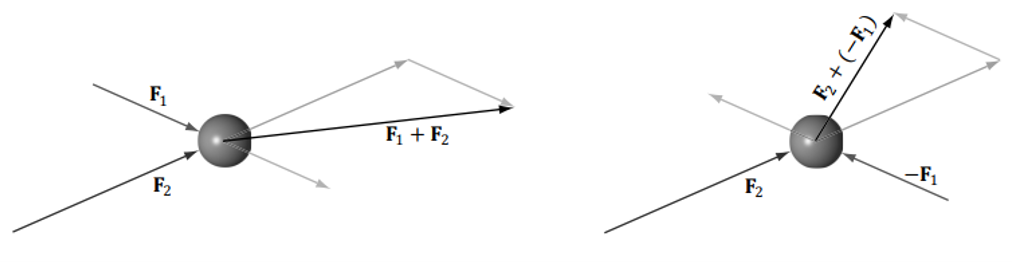
\includegraphics[width=\textwidth]{Images/4/4.Session.1.1.7}
                \caption{نیروهای اعمال شده به یک توپ. نیروها با استفاده از جمع بردار ترکیب می شوند تا نیروی برآیند به دست آید. \textbf{\vspace{10pt}}}
                \label{fig:4.Session.1.1.7}
            \end{figure}
        \end{example}
    \end{spacing}
}


\section{\textbf{بردارهای طول و واحد}}
{
    \Large
    \begin{spacing}{1.5}
        از نظر هندسی اندازه ی یک بردار، طول پاره خطی جهت دار است.
        اندازه ی یک بردار را با خط های عمودی دوتایی نشان می دهیم
        (به عنوان مثال، $\norm{u}$ اندازه ی $\textbf{u}$ را نشان می دهد).
        حالا با توجه به بردار $\textbf{u}=(x,y,z)$، می‌خواهیم بزرگی آن را به صورت جبری محاسبه کنیم.
        اندازه ی یک بردار سه بعدی را می توان با دو بار اعمال قضیه فیثاغورث محاسبه کرد.
        شکل \ref{fig:4.Session.1.1.8} را ببینید. ابتدا، ما به مثلث در صفحه xz با اضلاع x، z و وتر a نگاه می کنیم.

        \begin{figure}[H]
            \centering
            \setlength{\belowcaptionskip}{-10pt}
            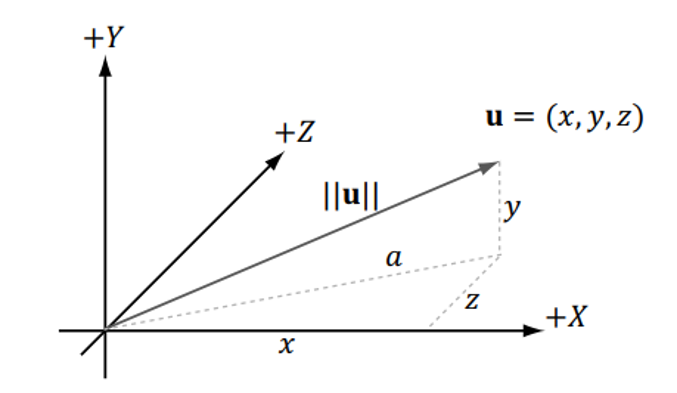
\includegraphics[width=0.5\textwidth]{Images/4/4.Session.1.1.8}
            \caption{طول سه بعدی یک بردار را می توان با دو بار اعمال قضیه فیثاغورث محاسبه کرد.}
            \label{fig:4.Session.1.1.8}
        \end{figure}

        از قضیه فیثاغورث، $a=\sqrt{\displaystyle x^2+z^2}$ داریم.
        حالا به مثلث با ضلع های \lr{a}، \lr{y} و وتر $\norm{u}$ نگاه کنید از قضیه فیثاغورث دوباره به فرمول اندازه ی زیر می رسیم:

        \begin{eqtn}{eqtn:1}
            \centering
            $\norm{\textbf{u}}=\sqrt{\displaystyle y^2+a^2}=\sqrt{\displaystyle y^2+(\sqrt{\displaystyle x^2+z^2})^2}=\sqrt{\displaystyle x^2+y^2+z^2}$
        \end{eqtn}

        برای برخی از استفاده ها، ما به طول یک بردار اهمیتی نمی دهیم زیرا می خواهیم از بردار برای نمایش یک جهت خالص استفاده کنیم.
        می خواهیم طول چنین بردارهایی با فقط یک جهت دقیقاً 1 باشد.
        وقتی طول واحد برداری را می سازیم، می گوییم که بردار را نرمال کرده ایم.
        می توانیم یک بردار را با تقسیم هر یک از اجزای بر بزرگی آن ، نرمال کنیم:

        \begin{eqtn}{eqtn:2}
            \centering
            $\hat{\textbf{u}}=\frac{\displaystyle\textbf{u}}{\displaystyle\norm{\textbf{u}}}=\left(\frac{\displaystyle x}{\displaystyle\norm{\textbf{u}}},
            \frac{\displaystyle y}{\displaystyle\norm{\textbf{u}}}, \frac{\displaystyle z}{\displaystyle\norm{\textbf{u}}}\right)$
        \end{eqtn}

        برای تأیید صحت این فرمول، می توانیم طول $\hat{\textbf{u}}$ را محاسبه کنیم

        \begin{center}
            $\norm{\hat{\textbf{u}}}=\sqrt{\displaystyle \left(\frac{\displaystyle x}{\displaystyle\norm{\textbf{u}}}\right)^2,
                \left(\frac{\displaystyle y}{\displaystyle\norm{\textbf{u}}}\right)^2,
                \left(\frac{\displaystyle z}{\displaystyle\norm{\textbf{u}}}\right)^2}=\frac{\displaystyle x^2+y^2+z^2}{\displaystyle\sqrt{\displaystyle \norm{\textbf{u}}^2}}
            =\frac{\displaystyle\norm{\textbf{u}}}{\displaystyle\norm{\textbf{u}}}=1$
        \end{center}

        پس \hat{\textbf{u}} در واقع یک بردار واحد است.

        \begin{example}{exp:3}
            بردار $\textbf{v}=(-1,3,4)$ را نرمال کنید. داریم $\norm{\textbf{v}}=\sqrt{\displaystyle (-1)^2+3^2+4^2}=\sqrt{\displaystyle 26}$. پس:

            \begin{center}
                $\hat{\textbf{v}}=\frac{\displaystyle\textbf{v}}{\displaystyle\norm{\textbf{v}}}=\left(-\frac{\displaystyle 1}{\displaystyle\sqrt{\displaystyle 26}},
                \frac{\displaystyle 3}{\displaystyle\sqrt{\displaystyle 26}}, \frac{\displaystyle 4}{\displaystyle\sqrt{\displaystyle 26}}\right)$
            \end{center}

            برای تأیید اینکه $\hat{\textbf{v}}$ واقعاً یک بردار واحد است، طول آن را محاسبه می کنیم:

            \begin{center}
                $\norm{\hat{\textbf{v}}}=\sqrt{\displaystyle \left(-\frac{\displaystyle 1}{\displaystyle\sqrt{\displaystyle 26}}\right)^2,
                    \left(\frac{\displaystyle 3}{\displaystyle\sqrt{\displaystyle 26}}\right)^2, \left(\frac{\displaystyle 4}{\displaystyle\sqrt{\displaystyle 26}}\right)^2}=
                \sqrt{\displaystyle\frac{\displaystyle 1}{\displaystyle 26}+\frac{\displaystyle 9}{\displaystyle 26}+\frac{\displaystyle 16}{\displaystyle 26}}=\sqrt{\displaystyle 1}=1$
            \end{center}
        \end{example}
    \end{spacing}
}


\section{\textbf{ضرب داخلی}}
\label{sec:3}
{
    \Large
    \begin{spacing}{1.5}
        ضرب نقطه ای (داخلی) شکلی از ضرب برداری است که منجر به یک مقدار اسکالر می شود.
        به همین دلیل، گاهی اوقات از آن به عنوان یک ضرب اسکالر یاد می شود.
        فرض کنید $\textbf{u}=(u_{x},u_{y},u_{z})$ و  $\textbf{v}=(v_{x},v_{y},v_{z})$،
        پس حاصل ضرب داخلی به صورت زیر تعریف می‌شود:

        \begin{eqtn}{eqtn:3}
            \centering
            \LARGE
            $\textbf{u}\cdot\textbf{v}=u_{x}v_{x}+u_{y}v_{y}+u_{z}v_{z}$
        \end{eqtn}

        به عبارت دیگر ، ضرب داخلی مجموع ضرب های اجزای مربوطه ست.

        همچنین تعریف ضرب داخلی معنای هندسی آشکاری ارائه نمی دهد.
        با استفاده از قانون کسینوس (به تمرین ***** مراجعه کنید)، می توانیم رابطه ای را پیدا کنیم که در آن $\theta$ زاویه بین بردارهای $\textbf{u}$ و $\textbf{v}$ است به طوری که $0\leq\theta\leq\pi$؛ شکل \ref{fig:4.Session.1.1.9} را ببینید.

        \begin{eqtn}{eqtn:4}
            \centering
            \LARGE
            $\textbf{u}\cdot\textbf{v}=\norm{\textbf{u}}\norm{\textbf{v}}\cos\theta$
        \end{eqtn}

        بنابراین، معادله \ref{eqtn:4} می گوید که حاصلضرب نقطه ای بین دو بردار، کسینوس زاویه بین آنها است که با بزرگی بردارها ضرب شده است.
        به خصوص، اگر هر دو بردار $\textbf{u}$ و $\textbf{v}$ بردار واحد باشند،
        آنگاه $\textbf{u}\cdot\textbf{v}$ کسینوس زاویه بین آنهاست (یعنی $\textbf{u}\cdot\textbf{v}=\cos\theta$).
        معادله \ref{eqtn:4} برخی از ویژگی های هندسی مفید ضرب داخلی را در اختیار ما قرار می دهد:

        \begin{figure}[H]
            \centering
            \setlength{\belowcaptionskip}{-10pt}
            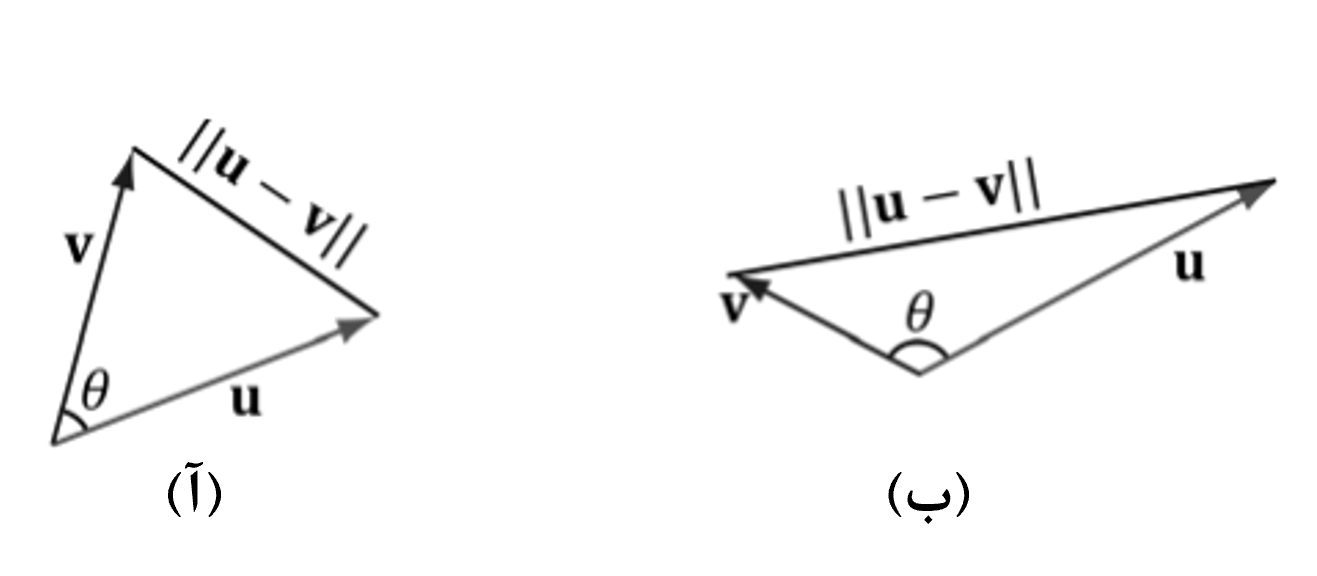
\includegraphics[width=0.8\textwidth]{Images/4/4.Session.1.1.9}
            \caption{در شکل سمت چپ، زاویه $\theta$ بین $\textbf{u}$ و $\textbf{v}$ یک زاویه تند است.
            در شکل سمت راست، زاویه $\theta$ بین $\textbf{u}$ و $\textbf{v}$ یک زاویه منفرجه (باز) است.
            وقتی به زاویه بین دو بردار اشاره می کنیم، همیشه منظورمان کوچکترین زاویه است،
            یعنی زاویه $\theta$ به طوری که $0\leq\theta\leq\pi$.}
            \label{fig:4.Session.1.1.9}
        \end{figure}

        \begin{enumerate}
            \item {اگر $\textbf{u}\cdot\textbf{v}=0$، در نتیجه $\textbf{u}\perp\textbf{v}$ (یعنی بردار ها بر هم عمودند).}
            \item {اگر $\textbf{u}\cdot\textbf{v}>0$، در نتیجه زاویه ی بین $\theta$ و دو بردار کمتر از 90 درجه ست (یعنی بردار ها با هم زاویه ی تند میسازند).}
            \item {اگر $\textbf{u}\cdot\textbf{v}<0$، در نتیجه زاویه ی بین $\theta$ و دو بردار بیشتر از 90 درجه ست (یعنی بردار ها با هم زاویه ی منفرجه میسازند).}
        \end{enumerate} \\

        \begin{example}{exp:4}
            فرض کنید $\textbf{u}=(1,2,3)$ و $\textbf{v}=(-4,0,-1)$ باشند. زوایه ی بین $\textbf{u}$ و $\textbf{v}$ را پیدا کنید. \\
            ابتدا موارد زیر را محاسبه میکنیم:

            \begin{center}
                $\textbf{u}\cdot\textbf{v}=(1,2,3)\cdot(-4,0,-1)=-4-3=-7$

                $\norm{\textbf{u}}=\sqrt{\displaystyle 1^2+2^2+3^2}=\sqrt{\displaystyle 14}$

                $\norm{\textbf{v}}=\sqrt{\displaystyle (-4)^2+0^2+(-1)^2}=\sqrt{\displaystyle 17}$
            \end{center}

            حالا ، معادله ی \ref{eqtn:4} را برای حل $\theta$ اعمال میکنیم:

            \begin{center}
                $\cos\theta=\frac{\displaystyle\textbf{u}\cdot\textbf{v}}{\displaystyle\norm{\textbf{v}}\norm{\textbf{u}}}=\frac{\displaystyle -7}{\displaystyle \sqrt{\displaystyle 14}\sqrt{\displaystyle 17}}$

                $\theta=\cos^-1\frac{\displaystyle -7}{\displaystyle \sqrt{\displaystyle 14}\sqrt{\displaystyle 17}}\thickapprox117^\circ$
            \end{center}
        \end{example}

        \textbf{\vspace{-6pt}}
        \begin{example}{exp:5}
            شکل \ref{fig:4.Session.1.1.10} را در نظر بگیرید.
            با توجه به $\textbf{v}$ و بردار واحد $\textbf{n}$، فرمولی برای $\textbf{p}$ بر حسب $\textbf{v}$ و $\textbf{n}$ با استفاده از ضرب داخلی پیدا کنید. \\
            ابتدا، از شکل مشاهده کنید که عدد اسکالر $\textbf{k}$ وجود دارد
            که $\textbf{p}=k\textbf{n}$؛ علاوه بر این، از آنجایی که ما $\norm{\textbf{u}}=1$ فرض کردیم،
            داریم $\norm{\textbf{p}}=\norm{k\textbf{n}}=\abs{k}\norm{\textbf{n}}=\abs{k}$.
            (توجه داشته باشید که $k$ ممکن است منفی باشد اگر و تنها اگر $\textbf{p}$ و $\textbf{n}$ در جهت مخالف قرار گیرند.)
            با استفاده از مثلثات، داریم که $k=\norm{\textbf{v}}\cos\theta$؛
            بنابراین، $\textbf{p}=k\textbf{n}=(\norm{\textbf{v}}\cos\theta)\textbf{n}$.
            با این حال، از آنجایی که \textbf{n} یک بردار واحد است، می توانیم این را به روش دیگری بگوییم:

            \begin{center}
                $\textbf{p}=(\norm{\textbf{v}}\cos\theta)\textbf{n}=(\norm{\textbf{v}}\cdot 1\cos\theta)\textbf{n}=(\norm{\textbf{v}}\norm{\textbf{n}}\cos\theta)\textbf{n}=(\textbf{v}\cdot\textbf{n})\textbf{n}$
            \end{center}

            به طور خاص، این $k=\textbf{v}\cdot\textbf{n}$ را نشان می دهد که تفسیر هندسی $\textbf{v}\cdot\textbf{n}$ را هنگامی که $\textbf{n}$ یک بردار واحد است، نشان می دهد. ما $\textbf{p}$ را تصویر متعامد/قائم (\lr{orthogonal projection}) $\textbf{v}$ روی $\textbf{n}$ می نامیم و معمولاً به شکل زیر نشان داده می شود:

            \begin{center}
                $\textbf{p}=proj_{n}(\textbf{v})$
            \end{center}

            اگر $\textbf{v}$ را به عنوان نیرو تعبیر کنیم، $\textbf{p}$ را می توان به عنوان بخشی از نیروی $\textbf{v}$ در نظر گرفت که در جهت $\textbf{n}$ عمل می کند.
            به همین ترتیب، بردار $\textbf{w}=perp_{n}(\textbf{v})=\textbf{v}-\textbf{p}$ بخشی از نیروی $\textbf{v}$ است که در جهت $\textbf{n}$ متعامد عمل می کند
            (به همین دلیل است که آن را با $perp_{n}(\textbf{v})$ برای عمود نشان می دهیم).
            مشاهده کنید که $\textbf{v}=\textbf{p}+\textbf{w}=proj_{n}(\textbf{v})+perp_{n}(\textbf{v})$ که می گوییم بردار $\textbf{v}$ را به مجموع دو بردار متعامد $\textbf{p}$ و $\textbf{w}$ تجزیه کرده ایم.

            اگر $\textbf{n}$ طول واحد نباشد، همیشه می‌توانیم ابتدا آن را نرمال کنیم تا طول آن را واحد کنیم.
            جایگزینی $\textbf{n}$ با بردار واحد $\frac{\displaystyle\textbf{n}}{\norm{\textbf{n}}}$ فرمول تصویر کلی تری را به ما می دهد:

            \begin{center}
                $\textbf{p}=proj_{n}(\textbf{v})=\left( \textbf{v}\cdot\frac{\displaystyle\textbf{n}}{\norm{\textbf{n}}} \right)\frac{\displaystyle\textbf{n}}{\norm{\textbf{n}}}=\frac{\displaystyle(\textbf{v}\cdot\textbf{n})}{\norm{\textbf{n}}^2}\textbf{n}$
            \end{center}

            \begin{figure}[H]
                \centering
                \setlength{\belowcaptionskip}{-10pt}
                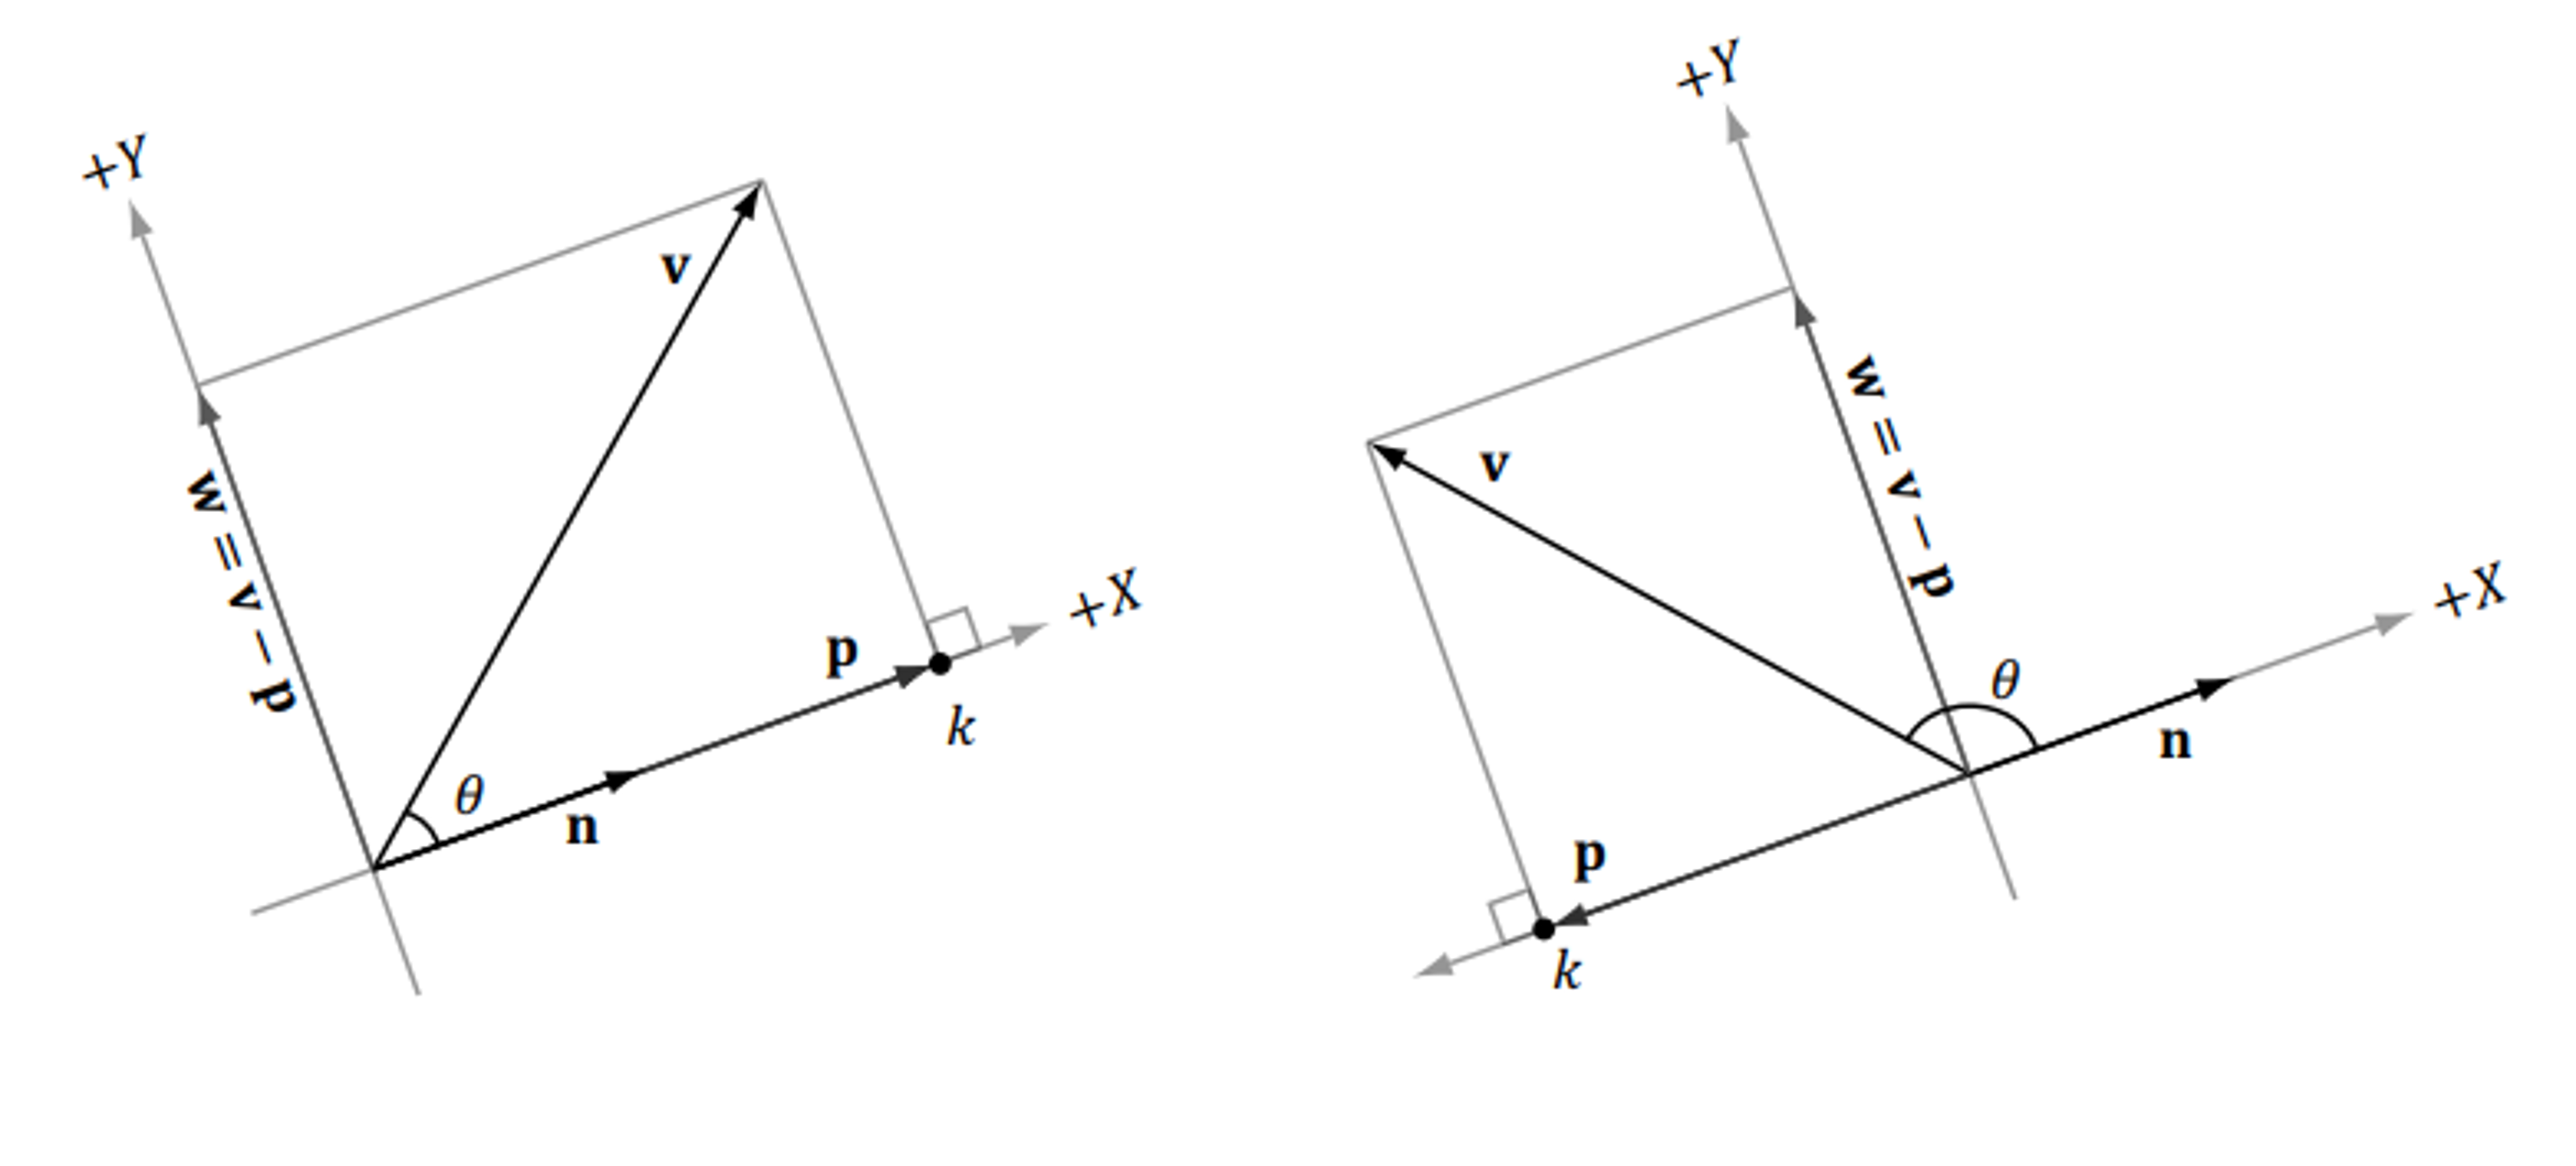
\includegraphics[width=0.5\textwidth]{Images/4/4.Session.1.1.10}
                \caption{تصویر متعامد/قائم $\textbf{v}$ روی $\textbf{n}$. \textbf{\vspace{10pt}}}
                \label{fig:4.Session.1.1.10}
            \end{figure}
        \end{example}
    \end{spacing}
}

\textbf{\vspace{-10pt}}

\subsection{\textbf{متعامد سازی}}
\label{sec:3.1}
{
    \Large
    \begin{spacing}{1.5}
        مجموعه ای از بردارها $\{\textbf{v}_{0},...,\textbf{v}_{n-1}\}$ متعامد نامیده می شود که بردارها همگی متعامد (هر بردار در مجموعه نسبت به هر بردار دیگری در مجموعه متعامد باشد) و طول واحد باشند.
        گاهی اوقات ما مجموعه ای از بردارها را داریم که تقریباً متعارف هستند، اما نه کاملاً.
        یک کار متداول این است که مجموعه را متعامد سازی کنید تا یک مجموعه ی متعامد شود.
        در گرافیک کامپیوتری سه بعدی ممکن است با یک مجموعه متعارف شروع کنیم، اما به دلیل مسائل مربوط به دقت عددی، مجموعه به تدریج غیرمتعارف شود.
        ما عمدتاً با موارد دو بعدی و سه بعدی این مشکل (یعنی مجموعه هایی که به ترتیب شامل دو و سه بردار هستند) سروکار داریم.

        ابتدا مورد دو بعدی ساده تر را بررسی می کنیم.
        فرض کنید مجموعه بردارهای $\{\textbf{v}_{0},\textbf{v}_{1}\}$ را داریم که می‌خواهیم آن‌ها را به یک مجموعه متعامد $\{\textbf{w}_{0},\textbf{w}_{1}\}$ تبدیل کنیم،
        همانطور که در شکل \ref{fig:4.Session.1.1.11} نشان داده شده است.
        ما با $\textbf{w}_{0}=\textbf{v}_{0}$ شروع کرده و $\textbf{v}_{1}$ را تغییر میدهیم تا آن را به $\textbf{w}_{0}$ متعامد کنیم.
        این کار با تفریق کردن بخشی از $\textbf{v}_{1}$ که در جهت $\textbf{w}_{0}$  عمل می کند، انجام می شود:

        \begin{center}
            $\textbf{w}_{1}=\textbf{v}_{1}-proj_{\textbf{w}_{0}}(\textbf{v}_{1})$
        \end{center}

        اکنون مجموعه ای متعامد از بردارها داریم $\{\textbf{w}_{0},\textbf{w}_{1}\}$.
        آخرین مرحله برای ساخت مجموعه متعارف نرمال کردن $\textbf{w}_{0}$ و $\textbf{w}_{1}$ برای ایجاد طول واحد است.

        \begin{figure}[H]
            \centering
            \setlength{\belowcaptionskip}{-10pt}
            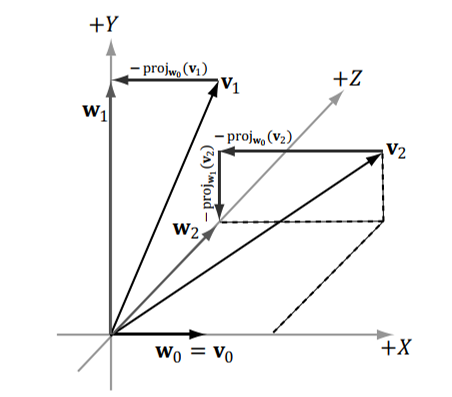
\includegraphics[width=0.5\textwidth]{Images/4/4.Session.1.1.11}
            \caption{متعامد سازی دو بعدی}
            \label{fig:4.Session.1.1.11}
        \end{figure}

        حالت سه بعدی به همان شکل مورد دو بعدی اما با مراحل بیشتر است.
        فرض کنید مجموعه بردارهای $\{\textbf{v}_{0},\textbf{v}_{1},\textbf{v}_{2}\}$ را داریم که می‌خواهیم آنها را یک مجموعه متعامد $\{\textbf{w}_{0},\textbf{w}_{1},\textbf{w}_{2}\}$ کنیم، مطابق شکل \ref{fig:4.Session.1.1.12}.
        ما با $\textbf{w}_{0}=\textbf{v}_{0}$ شروع می کنیم و $\textbf{v}_{1}$ را تغییر می دهیم تا به $\textbf{w}_{0}$ متعامد شود.
        این کار با کم کردن بخشی از $\textbf{v}_{1}$ که در جهت $\textbf{w}_{0}$ عمل می کند انجام می شود:

        \begin{center}
            $\textbf{w}_{1}=\textbf{v}_{1}-proj_{\textbf{w}_{0}}(\textbf{v}_{1})$
        \end{center}

        \begin{figure}[H]
            \centering
            \setlength{\belowcaptionskip}{-10pt}
            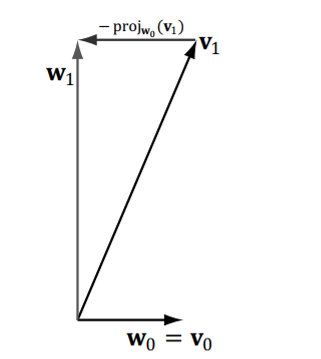
\includegraphics[width=0.35\textwidth]{Images/4/4.Session.1.1.12}
            \caption{متعامد سازی سه بعدی}
            \label{fig:4.Session.1.1.12}
        \end{figure}

        در مرحله بعد، $\textbf{v}_{2}$ را تغییر می دهیم تا آن را متعامد به $\textbf{w}_{0}$ و $\textbf{w}_{1}$ کنیم.
        این کار با تفریق کردن بخشی از $\textbf{v}_{2}$ که در جهت $\textbf{w}_{0}$ عمل می کند و بخشی از $\textbf{v}_{2}$ که در جهت $\textbf{w}_{1}$ عمل می کند، انجام می شود:

        \begin{center}
            $\textbf{w}_{2}=\textbf{v}_{2}-proj_{\textbf{w}_{0}}(\textbf{v}_{2})-proj_{\textbf{w}_{1}}(\textbf{v}_{2})$
        \end{center}

        اکنون یک مجموعه متعامد از بردارها داریم $\{\textbf{w}_{0},\textbf{w}_{1},\textbf{w}_{2}\}$.
        آخرین مرحله برای ساخت مجموعه متعامد نرمال کردن $\textbf{w}_{0}$، $\textbf{w}_{1}$ و $\textbf{w}_{2}$ است تا طول آنها را واحد کنیم.

        برای حالت کلی $\textbf{n}$ بردار $\{\textbf{v}_{0},...,\textbf{v}_{n-1}\}$ که می‌خواهیم آنها را به یک مجموعه متعامد تبدیل کنیم $\{\textbf{w}_{0},...,\textbf{w}_{n-1}\}$، ما روال زیر را داریم که معمولاً فرآیند متعامدسازی گرام اشمیت (\lr{Gram-Schmidt}) نامیده می شود:

        \begin{center}
            گام پایه: $\textbf{w}_{0}=\textbf{v}_{0}$ قرار میدهیم

            به ازای $1\leq i\leq n-1$ ، \\ $\textbf{w}_{i}=\textbf{v}_{i}-\sum_{j=1}^{i-1}proj_{\textbf{w}_{j}}(\textbf{v}_{i})$ قرار میدهیم

            گام نرمال سازی: $\textbf{w}_{i}=\frac{\displaystyle\textbf{w}_{i}}{\displaystyle\norm{\textbf{w}_{i}}}$ قرار میدهیم
        \end{center}

        دوباره، ایده شهودی این است که وقتی یک بردار $\textbf{v}_{i}$ را از مجموعه ورودی انتخاب می کنیم تا به مجموعه متعارف اضافه کنیم،
        باید اجزای $\textbf{v}_{i}$ را که در جهت بردارهای دیگر عمل کرده و از قبل در مجموعه متعامد قرار دارند ($\textbf{w}_{0},\textbf{w}_{1},...,\textbf{w}_{i-1}$) را کم کنیم.
        این کار باعث اطمینان حاصل از این که بردار جدید اضافه شده با سایر بردارهای موجود در مجموعه متعامد، متعامد باشد، میشود.
    \end{spacing}
}


\section{\textbf{ضرب خارجی}}
{
    \Large
    \begin{spacing}{1.5}
        شکل دوم بردار ضرب ریاضی، ضرب خارجی است.
        بر خلاف ضرب داخلی که به یک اسکالر ختم می‌شود، ضرب خارجی به یک بردار دیگر ختم می‌شود.
        علاوه بر این، ضرب خارجی فقط برای بردارهای سه بعدی تعریف شده است (در واقع ضرب خارجی دو بعدی وجود ندارد).
        با ضرب خارجی دو بردار سه بعدی u و v، بردار دیگری به دست می‌آید،که w متعامد به u و v است.
        شکل \ref{fig:4.Session.1.1.13} را ببینید.
        اگر $\textbf{u}=(u_{x},u_{y},u_{z})$ و  $\textbf{v}=(v_{x},v_{y},v_{z})$ باشد، آنگاه ضرب خارجی به این صورت محاسبه می‌شود:

        \begin{eqtn}{eqtn:5}
            \centering
            $\textbf{w}=\textbf{u}\times\textbf{v}=(u_{y}v_{z}-u_{z}v_{y}, u_{z}v_{x}-u_{x}v_{z}, u_{x}v_{y}-u_{y}v_{z})$
        \end{eqtn}

        \begin{point}{pnt:4}
            \Large
            اگر در سیستم مختصات راستگرد کار می کنید، پس از قانون شست دست راست استفاده می کنید:
            اگر دست راست خود را طوری بگیرید که انگشتان در جهت بردار اول u باشد و سپس انگشتان خود را به سمت v با زاویه ی $0\leq\theata\leq \pi$ خم کنید، انگشت شست شما در جهت $\textbf{w}=\textbf{u}\times\textbf{v}$ قرار می گیرد.
        \end{point}

        \begin{figure}[H]
            \centering
            \setlength{\belowcaptionskip}{-10pt}
            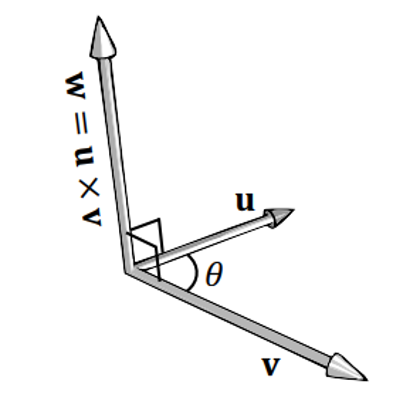
\includegraphics[width=0.35\textwidth]{Images/4/4.Session.1.1.13}
            \caption{ضرب خارجی دو بردار سه بعدی $\textbf{u}$ و $\textbf{v}$ بردار دیگر $\textbf{w}$ را به دست می آورد که متعامد با $\textbf{u}$ و $\textbf{v}$ است.
            اگر دست چپ خود را طوری بگیرید که انگشتان در جهت بردار اول u باشد و سپس انگشتان خود را به سمت v با زاویه ی $0\leq\theata\leq \pi$ خم کنید، انگشت شست شما در جهت $\textbf{w}=\textbf{u}\times\textbf{v}$ قرار می گیرد. به این قانون شست چپ می گویند.}
            {متعامد سازی سه بعدی}
            \label{fig:4.Session.1.1.13}
        \end{figure}

        \begin{example}{exp:6}
            فرض کنید $\textbf{u}=(1,2,3)$ و $\textbf{v}=(1,2,3)$ باشد. سپس $\textbf{w}=\textbf{u}\times\textbf{v}$ و $\textbf{z}=\textbf{v}\times\textbf{z}$ را محاسبه کنید. معادله ی \ref{eqtn:5} را اعمال میکنیم: \\
            \begin{equation*}
                \centering
                \begin{split}
                    \textbf{w}&=\textbf{u}\times\textbf{v}\\
                    &=(2,1,3)\times(2,0,0)\\
                    &=(1\cdot 0-3\cdot 0, 3\cdot 2-2\cdot 0, 2\cdot 0-1\cdot 2)\\
                    &=(0,6,-2)
                \end{split}
            \end{equation*}
            و
            \begin{equation*}
                \centering
                \begin{split}
                    \textbf{z}&=\textbf{v}\times\textbf{u}\\
                    &=(2,0,0)\times(2,1,3)\\
                    &=(0\cdot 3-0\cdot 1, 0\cdot 2-2\cdot 3, 2\cdot 1-0\cdot 2)\\
                    &=(0,6,-2)
                \end{split}
            \end{equation*}

            این نتیجه یک چیز را روشن می کند، به طور کلی $\textbf{u}\times\textbf{v}\neq\textbf{v}\times\textbf{u}$. بنابراین، می گوییم که ضرب خارجی خاصیت جابجایی ندارد.
            در واقع می توان نشان داد که $\textbf{u}\times\textbf{v}=-\textbf{v}\times\textbf{u}$. شما می توانید بردار به دست آمده از ضرب خارجی را با قانون انگشت شست چپ تعیین کنید.
            اگر ابتدا انگشتان خود را در جهت بردار اول نشانه بگیرید و سپس انگشتان خود را به سمت بردار دوم خم کنید (همیشه مسیر را با کوچکترین زاویه انتخاب کنید)، همانطور که در شکل \ref{fig:4.Session.1.1.11} نشان داده شده است، انگشت شست شما در جهت بردار حاصل قرار می گیرد.

            برای نشان دادن اینکه $\textbf{w}$ متعامد به $\textbf{u}$ و $\textbf{w}$ متعامد بر $\textbf{v}$ است،
            از بخش \ref{sec:3} یادآوری می کنیم که اگر$\textbf{u}\times\textbf{v}=0$ باشد،
            آنگاه $\textbf{u}\perp\textbf{v}$ است (یعنی بردارها متعامد هستند). زیرا

            \begin{center}
                $\textbf{w}\times\textbf{u}=(0,6,-2)\cdot(2,1,3)=0\cdot 2+6\cdot 1+(-2)\cdot 3=0$

                و

                $\textbf{w}\times\textbf{v}=(0,6,-2)\cdot(2,0,0)=0\cdot 2+6\cdot 0+(-2)\cdot 0=0$
            \end{center}

            نتیجه می گیریم که $\textbf{w}$ متعامد به $\textbf{u}$ و $\textbf{w}$ متعامد بر $\textbf{v}$ است.
        \end{example}
    \end{spacing}
}

\subsection{\textbf{ضرب خارجی شبه دو بعدی}}
{
    \Large
    \begin{spacing}{1.5}
        ضرب خارجی به ما امکان می دهد یک بردار متعامد به دو بردار سه بعدی داده شده را پیدا کنیم.
        در دوبعدی وضعیت مشابهی نداریم،
        اما با توجه به بردار دوبعدی $\textbf{u}=u_{x},u_{y}$ پیدا کردن بردار $\textbf{v}$ متعامد به $\textbf{u}$ می‌تواند مفید باشد.
        شکل \ref{fig:4.Session.1.1.14} شکل هندسی ای را نشان می دهد که از آن $\textbf{v}=-u_{y},u_{x}$ پیدا میشود.
        اثبات آن ساده است:

        \begin{center}
            $\textbf{u}\cdot\textbf{v}=(u_{x},u_{y})\cdot(-u_{y},u_{x})=-u_{x}u_{y}+u_{y}u_{x}=0$
        \end{center}

        بنابراین $\textbf{u}\perp\textbf{v}$.
        مشاهده کنید که $\textbf{u}\cdot-\textbf{v}=u_{x}u_{y}+u_{y}(-u_{x})=0$، بنابراین $\textbf{u}\perp-\textbf{v}$ را نیز داریم.

        \begin{figure}[H]
            \centering
            \setlength{\belowcaptionskip}{-10pt}
            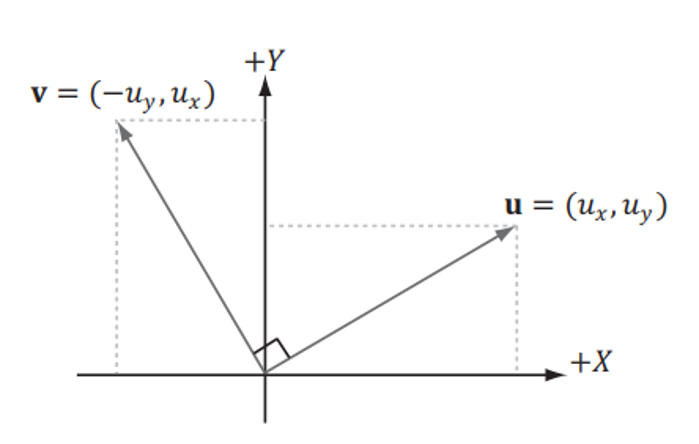
\includegraphics[width=0.5\textwidth]{Images/4/4.Session.1.1.14}
            \caption{ضرب خارجی شبه دوبعدی یک بردار $\textbf{u}$ به بردار متعامد $\textbf{v}$ ختم می شود.}
            \label{fig:4.Session.1.1.14}
        \end{figure}
    \end{spacing}
}

\subsection{\textbf{متعامد سازی با ضرب خارجی}}
{
    \Large
    \begin{spacing}{1.5}
        در بخش \ref{sec:3.1}، ما روشی برای متعامد کردن مجموعه ای از بردارها با استفاده از فرآیند گرام اشمیت را مشاهده کردیم.
        برای سه بعدی، استراتژی دیگری برای متعامد کردن مجموعه ای از بردارها $\textbf{v}_{0},\textbf{v}_{1},\textbf{v}_{2}$ وجود دارد که متعارف هستند،
        اما ممکن است به دلیل خطاهای انباشته شده در دقت عددی با استفاده از ضرب خارجی، غیرمتعارف شوند.
        برای شکل هندسی این فرآیند به شکل \ref{fig:4.Session.1.1.15} مراجعه کنید:

        \begin{enumerate}
            \item {$\textbf{w}_{0}=\frac{\displaystyle\textbf{v}_{0}}{\displaystyle\norm{\textbf{v}_{0}}}$ قرار میدهیم}
            \item {$\textbf{w}_{2}=\frac{\displaystyle\textbf{w}_{0}\times\textbf{v}_{1}}{\displaystyle\norm{\textbf{w}_{0}\times\textbf{v}_{1}}}$ قرار میدهیم}
            \item {با قرار دادن $\textbf{w}_{1}=\textbf{w}_{2}\times\textbf{w}_{0}$ توسط تمرین ******، $\norm{\textbf{w}_{2}\times\textbf{w}_{0}}=1$ زیرا $\textbf{w}_{2}\perp\textbf{w}_{0}$ و $\norm{\textbf{w}_{2}}=\norm{\textbf{w}_{0}}=1$،
            بنابراین در این مرحله آخر نیازی به نرمال سازی نداریم.}
        \end{enumerate}

        در این مرحله، مجموعه بردارهای $\{\textbf{w}_{0},\textbf{w}_{1},\textbf{w}_{2}\}$ متعامد است.

        \begin{figure}[H]
            \centering
            \setlength{\belowcaptionskip}{-10pt}
            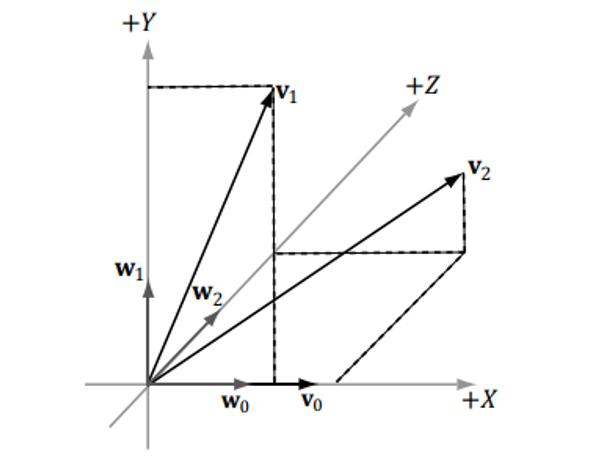
\includegraphics[width=0.5\textwidth]{Images/4/4.Session.1.1.15}
            \caption {متعامد سازی سه بعدی با ضرب خارجی}
            \label{fig:4.Session.1.1.15}
        \end{figure}

        \begin{point}{pnt:5}
            \Large
            در مثال بالا، ما با $\textbf{w}_{0}=\frac{\displaystyle\textbf{v}_{0}}{\displaystyle\norm{\textbf{v}_{0}}}$ شروع کردیم، به این معنی که هنگام رفتن از $\textbf{v}_{0}$ به $\textbf{w}_{0}$ جهت را تغییر ندادیم،
            ما فقط طول را تغییر دادیم.
            با این حال، جهت های $\textbf{w}_{1}$ و $\textbf{w}_{2}$ می تواند به ترتیب با $\textbf{v}_{1}$ و $\textbf{v}_{2}$ متفاوت باشد.
            بسته به کاربرد خاص، برداری که شما انتخاب میکنید تغییر جهت ندهد ممکن است مهم باشد.
            به عنوان مثال، در ادامه این کتاب، جهت دوربین را با سه بردار متعامد $\{\textbf{v}_{0},\textbf{v}_{1},\textbf{v}_{2}\}$ نشان می‌دهیم که بردار سوم $\textbf{v}_{2}$ جهتی را که دوربین به آن نگاه می‌کند، تعریف میکند.
            هنگامی که این بردارها را متعامد می کنیم، اغلب نمی خواهیم جهت مورد نظر خود را تغییر دهیم،
            بنابراین الگوریتم فوق را با $\textbf{v}_{2}$ شروع می کنیم و $\textbf{v}_{0}$ و $\textbf{v}_{1}$ را تغییر می دهیم تا بردارها متعامد شوند.
        \end{point}
    \end{spacing}
}

\section{\textbf{نقاط}}
{
    \Large
    \begin{spacing}{1.5}
        تاکنون در مورد بردارها بحث کرده ایم که موقعیت ها را توصیف نمی کنند.
        با این حال، ما همچنین باید موقعیت هایی را در برنامه های سه بعدی خود مشخص کنیم،
        به عنوان مثال، موقعیت هندسی سه بعدی و موقعیت دوربین مجازی سه بعدی.
        نسبت به یک سیستم مختصات، می‌توانیم از یک بردار در موقعیت استاندارد (شکل \ref{fig:4.Session.1.1.16}) برای نمایش یک موقعیت سه بعدی در فضا استفاده کنیم.
        ما این بردار را بردار موقعیت می نامیم.
        در این حالت، محل نوک بردار مشخصه مورد نظر است، نه جهت یا بزرگی.
        ما از عبارات "بردار موقعیت" و "نقطه" به جای یکدیگر استفاده خواهیم کرد زیرا بردار موقعیت برای شناسایی یک نقطه کافی است.

        \begin{figure}[H]
            \centering
            \setlength{\belowcaptionskip}{-10pt}
            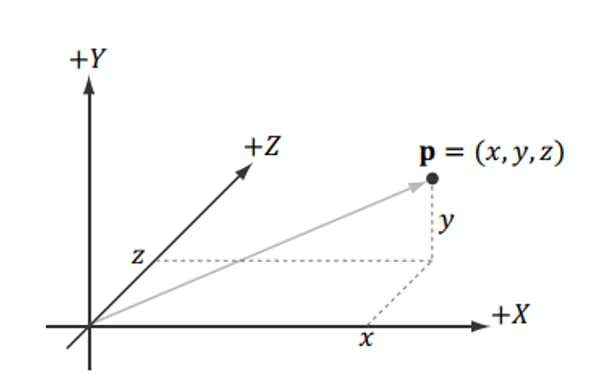
\includegraphics[width=0.5\textwidth]{Images/4/4.Session.1.1.16}
            \caption {بردار موقعیت، که از مبدا تا نقطه کشیده میشود، به طور کامل محل قرارگیری نقطه را نسبت به سیستم مختصات توصیف می کند.}
            \label{fig:4.Session.1.1.16}
        \end{figure}

        یکی از مزایای استفاده از بردارها برای نشان دادن نقاط، به ویژه در کد، این است که می‌توانیم عملیات های بردار را انجام دهیم که برای نقاط معنی ندارد.
        به عنوان مثال، از نظر هندسی، مجموع دو نقطه باید به چه معنا باشد؟
        از سوی دیگر، برخی از عملیات را می توان به نقاط گسترش داد.
        به عنوان مثال، ما فاصله ی دو نقطه $\textbf{q}-\textbf{p}$ را برداری از $\textbf{p}$ به $\textbf{q}$ تعریف می کنیم. همچنین، ما یک نقطه $\textbf{p}$ به اضافه بردار $\textbf{v}$ را نقطه ی $\textbf{q}$ تعریف میکنیم که با جابجایی p با بردار v به دست می آید.
        به راحتی، از آنجایی که ما از بردارها برای نشان دادن نقاط نسبت به یک سیستم مختصات استفاده می‌کنیم، نیازی به کار اضافی برای عملیات نقطه‌ای که قبلاً در مورد آن بحث شد، نیست، زیرا چارچوب جبر برداری از قبل آنها را آماده می‌کند. شکل \ref{fig:4.Session.1.1.16} را ببینید.

        \begin{figure}[H]
            \centering
            \setlength{\belowcaptionskip}{-10pt}
            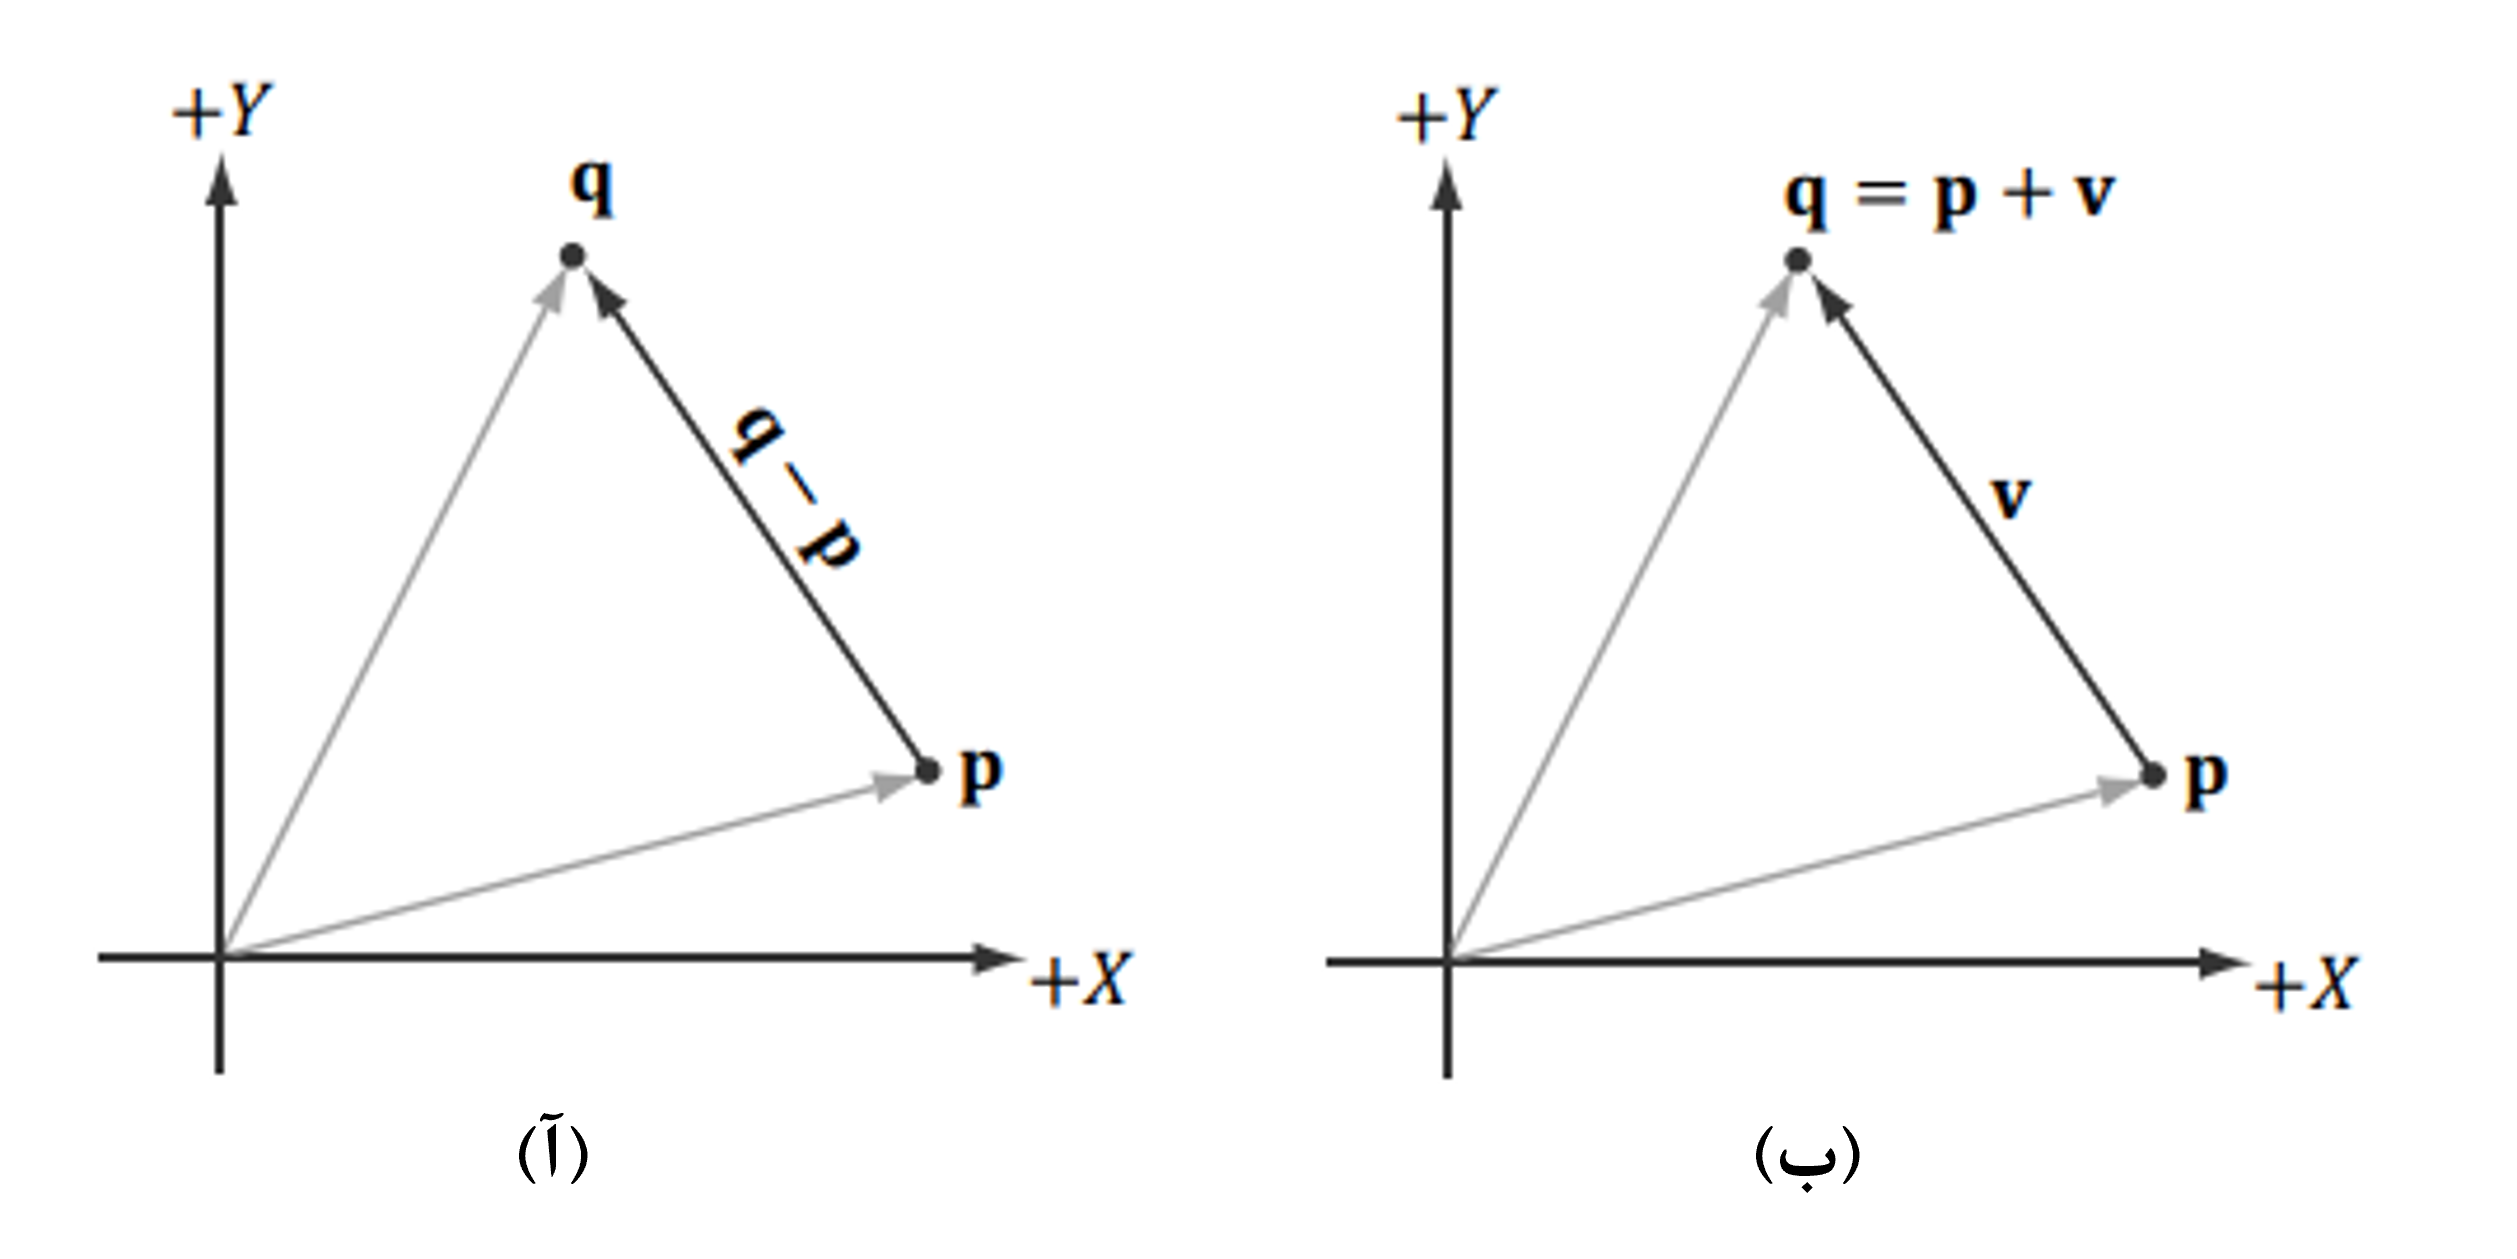
\includegraphics[width=0.5\textwidth]{Images/4/4.Session.1.1.17}
            \caption {(آ) فاصله ی دو نقطه $\textbf{q}-\textbf{p}$ برداری از $\textbf{p}$ به $\textbf{q}$ تعریف میشود. (ب) یک نقطه $\textbf{p}$ به اضافه بردار $\textbf{v}$ را نقطه ی $\textbf{q}$ تعریف میکنیم که با جابجایی p با بردار v به دست می آید.}
            \label{fig:4.Session.1.1.17}
        \end{figure}

        \begin{point}{pnt:6}
            \Large
            در واقع یک روش هندسی معنادار برای تعریف یک مجموع ویژه از نقاط وجود دارد که به آن ترکیب وابسته می گویند، که مانند میانگین وزنی نقاط است.
        \end{point}
    \end{spacing}
}

\section{\textbf{بردار های ریاضی \lr{DirectX}}}
{
    \Large
    \begin{spacing}{1.5}
        در ویندوز 8 و بالاتر، \lr{DirectX Math} یک کتابخانه ریاضی سه بعدی برای برنامه \lr{Direct3D} است که بخشی از \lr{Windows SDK} است.
        این کتابخانه از مجموعه دستورالعمل \lr{SSE2} (\lr{Streaming SIMD Extensions 2}) استفاده می کند.
        با رجیسترهای \lr{SIMD} گسترده \lr{128} بیتی (داده‌های چندگانه تک دستورالعمل)، دستورالعمل‌های \lr{SIMD} می‌توانند روی چهار عدد \lr{int} یا عدد \lr{float} \lr{32} بیتی با یک دستورالعمل کار کنند.
        این برای محاسبات برداری بسیار مفید است. برای مثال، اگر به جمع برداری نگاه کنید:

        \begin{center}
            $\textbf{u}+\textbf{v}=(u_{x}+v_{x},u_{y}+v_{y},u_{z}+v_{z})$
        \end{center}

        می بینیم که ما فقط اجزای مربوطه را اضافه می کنیم.
        با استفاده از \lr{SIMD} می‌توانیم به جای چهار دستور اسکالر، جمع بردار چهار بعدی را با یک دستور \lr{SIMD} انجام دهیم.
        اگر ما فقط به سه مختصات برای کار سه بعدی نیاز داشته باشیم، همچنان می توانیم از \lr{SIMD} استفاده کنیم، اما مختصات چهارم را نادیده می گیریم.
        به همین ترتیب، برای دو بعدی، مختصات سوم و چهارم را نادیده می گیریم.

        پوشش ما از کتابخانه ریاضی \lr{DirectX} جامع نیست و ما فقط بخش های کلیدی مورد نیاز برای این کتاب را پوشش می دهیم.
        برای تمام جزئیات، ما مستندات آنلاین [\lr{DirectXMath}] را توصیه می کنیم.
        برای خوانندگانی که مایلند بدانند چگونه یک کتابخانه برداری \lr{SIMD} ممکن است به طور بهینه توسعه یابد، و شاید درک کنند که چرا کتابخانه ریاضی \lr{DirectX} برخی از تصمیمات طراحی را اتخاذ کرده است،
        مقاله \lr{Designing Fast Cross-Platform SIMD Vector Libraries [by Oliveira2010]} را توصیه می کنیم.

        برای استفاده از کتابخانه ریاضی \lr{DirectX}، باید \lr{\texttt{\#include <DirectXMath.h>}} و برای برخی از انواع داده های اضافی \lr{\texttt{\#include <DirectXPackedVector.h>}} را وارد کنید.
        هیچ فایل کتابخانه ای اضافی وجود ندارد، زیرا تمام کدها به صورت درون خطی در فایل هدر پیاده سازی می شوند.
        کد \lr{DirectXMath.h} در فضای نام \texttt{DirectX} و کد \lr{DirectXPackedVector.h} در فضای نام \texttt{DirectX::PackedVector} وجود دارد.
        علاوه بر این، برای پلتفرم \lr{x86} باید \lr{SSE2} را فعال کنید:

        \begin{flushleft}
            \lr{\textbf{Project Properties > Configuration Properties > C/C++ > Code Generation > Enable Enhanced Instruction Set}}
        \end{flushleft}

        و برای همه پلتفرم‌ها باید مدل ممیز شناور سریع \lr{/fp:fast} را فعال کنید:

        \begin{flushleft}
            \lr{\textbf{Project Properties > Configuration Properties > C/C++ > Code Generation > Floating Point Model}}
        \end{flushleft}

        شما نیازی به فعال کردن \lr{SSE2} برای پلتفرم \lr{x64} ندارید زیرا تمام پردازنده‌های \lr{x64} از \lr{SSE2} (\url{http://en.wikipedia.org/wiki/SSE2}) پشتیبانی می‌کنند.
    \end{spacing}
}

\subsection{\textbf{انواع بردارها}}
{
    \Large
    \begin{spacing}{1.5}
        در \lr{DirectX Math}، نوع بردار هسته \texttt{XMVECTOR} است که به رجیسترهای سخت افزاری \lr{SIMD} نگاشت می شود.
        این یک نوع \lr{128} بیتی است که می تواند چهار \lr{float} \lr{32} بیتی را با یک دستورالعمل \lr{SIMD} پردازش کند.
        وقتی \lr{SSE2} در دسترس باشد، برای پلتفرم‌های \lr{x86} و \lr{x64} به این صورت تعریف می‌شود که \lr{\_\_m128} یک نوع \lr{SIMD} خاص است.:

        \begin{flushleft}
            \lr{\texttt{typedef \_\_m128 XMVECTOR;}}
        \end{flushleft}

        هنگام انجام محاسبات، بردارها باید از این نوع باشند تا از \lr{SIMD} استفاده کنند.
        همانطور که قبلا ذکر شد، ما همچنان از این نوع برای بردارهای دو بعدی و سه بعدی استفاده می کنیم تا از مزایای \lr{SIMD} استفاده کنیم،
        اما فقط اجزای استفاده نشده را صفر کرده و آنها را نادیده می گیریم.

        \texttt{XMVECTOR} باید \lr{16} بایت تراز شود و این به طور خودکار برای متغیرهای محلی و سراسری انجام می شود.
        برای اعضای داده کلاس، توصیه می شود به جای آن از \texttt{XMFLOAT2} (\lr{2D})، \texttt{XMFLOAT3} (\lr{3D}) و \texttt{XMFLOAT4} (\lr{4D}) استفاده کنید. این ساختارها در زیر تعریف می شوند:
        \textbf{\vspace{6pt}}
        \lr{\lstinputlisting[language=C++, caption=\rl{انواع بردار ها}, firstline=0, lastline=51]{Codes/main.c}}
        \textbf{\vspace{6pt}}
        اما اگر مستقیماً از این انواع برای محاسبات استفاده کنیم، از \lr{SIMD} استفاده نخواهیم کرد.
        برای استفاده از \lr{SIMD} باید نمونه هایی از این نوع را به نوع \texttt{XMVECTOR} تبدیل کنیم.
        این کار با توابع بارگیری ریاضی \lr{DirectX} انجام می شود.
        برعکس، \lr{DirectX} توابع ذخیره سازی را فراهم می کند که برای تبدیل داده ها از \texttt{XMVECTOR} به انواع \texttt{XMFLOATn} در بالا استفاده می شود.

        به طور خلاصه،

        \begin{enumerate}
            \item {از \texttt{XMVECTOR} برای متغیرهای محلی یا سراسری استفاده کنید.}
            \item {از \texttt{XMFLOAT2}، \texttt{XMFLOAT3} و \texttt{XMFLOAT4} برای اعضای داده کلاس استفاده کنید.}
            \item {قبل از انجام محاسبات از توابع بارگذاری برای تبدیل از \texttt{XMFLOATn} به \texttt{XMVECTOR} استفاده کنید.}
            \item {محاسبات را با نمونه های \texttt{XMVECTOR} انجام دهید.}
            \item {از توابع ذخیره سازی برای تبدیل از \texttt{XMVECTOR} به \texttt{XMFLOATn} استفاده کنید.}
        \end{enumerate}
    \end{spacing}
}

\subsection{\textbf{روش های بارگیری و ذخیره سازی}}
{
    \Large
    \begin{spacing}{1.5}
        ما از روش های زیر برای بارگذاری داده ها از \texttt{XMFLOATn} در \texttt{XMVECTOR} استفاده می کنیم:
        \textbf{\vspace{4pt}}
        \lr{\lstinputlisting[language=C++, caption=\rl{بارگیری}, firstline=55, lastline=62]{Codes/main.c}}
        \textbf{\vspace{3pt}}
        ما از روش های زیر برای ذخیره داده ها از \texttt{XMVECTOR} در \texttt{XMFLOATn} استفاده می کنیم:
        \textbf{\vspace{4pt}}
        \lr{\lstinputlisting[language=C++, caption=\rl{ذخیره سازی}, firstline=66, lastline=73]{Codes/main.c}}
        \textbf{\vspace{3pt}}
        توابع \lr{getter} و \lr{setter} برای دریافت یا تنظیم یک جزء \texttt{XMVECTOR} استفاده میشوند:
        \textbf{\vspace{4pt}}
        \lr{\lstinputlisting[language=C++, caption={Setter \& Getter}, firstline=77, lastline=84]{Codes/main.c}}
    \end{spacing}
}

\textbf{\vspace{-65pt}}
\subsection{\textbf{ارسال پارامتر}}
{
    \Large
    \begin{spacing}{1.5}
        برای اهداف کارایی، مقادیر \texttt{XMVECTOR} را می توان به عنوان آرگومان به توابع در ثبات های \lr{SSE/SSE2} به جای روی پشته ارسال کرد.
        تعداد آرگومان هایی که می توان از این طریق عبور داد به پلتفرم (به عنوان مثال ویندوز \lr{32} بیتی، ویندوز \lr{64} بیتی و ویندوز \lr{RT}) و کامپایلر بستگی دارد.
        بنابراین، برای مستقل بودن از پلتفرم/کامپایلر، از انواع \texttt{FXMVECTOR}، \texttt{GXMVECTOR}، \texttt{HXMVECTOR} و \texttt{CXMVECTOR} برای عبور پارامترهای \texttt{XMVECTOR} استفاده می‌کنیم.
        اینها بر اساس پلتفرم و کامپایلر به نوع مناسبی تعریف می شوند.
        علاوه بر این، حاشیه نویسی کنوانسیون فراخوانی \texttt{XM\_CALLCONV} باید قبل از نام تابع مشخص شود تا از قرارداد فراخوانی مناسب استفاده شود،
        که باز هم به نسخه کامپایلر بستگی دارد.

        قوانین عبور پارامترهای \texttt{XMVECTOR} به شرح زیر است:
        \begin{enumerate}
            \item {سه پارامتر اول \texttt{XMVECTOR} باید از نوع \texttt{FXMVECTOR} باشند.}
            \item {\texttt{XMVECTOR} چهارم باید از نوع \texttt{GXMVECTOR} باشد.}
            \item {پنجمین و ششمین پارامتر \texttt{XMVECTOR} باید از نوع \texttt{HXMVECTOR} باشد.}
            \item {هر پارامتر اضافی \texttt{XMVECTOR} باید از نوع \texttt{CXMVECTOR} باشد.}
        \end{enumerate}

        نحوه تعریف این انواع در ویندوز \lr{32} بیتی را با کامپایلری که از قرارداد \texttt{\_\_fastcall} پشتیبانی می کند و
        کامپایلری که از قرارداد فراخوانی \texttt{\_\_vectorcall} جدیدتر پشتیبانی می کند، توضیح می دهیم:
        \textbf{\vspace{6pt}}
        \lr{\lstinputlisting[language=C++, firstline=88, lastline=100]{Codes/main.c}}
        \textbf{\vspace{6pt}}
        برای جزئیات نحوه تعریف این انواع برای سایر پلتفرم‌ها، به \lr{«Calling Conventions»} در بخش \lr{«Internals Library»} در مستندات \lr{DirectX Math} مراجعه کنید.
        استثنای این قوانین مربوط به متدهای سازنده است. [\lr{DirectXMath}] توصیه می کند هنگام نوشتن سازنده ای که پارامترهای \texttt{XMVECTOR} را می گیرد،
        از \texttt{FXMVECTOR} برای سه پارامتر اول \texttt{XMVECTOR} و \texttt{CXMVECTOR} برای بقیه استفاده کنید.
        علاوه بر این، از حاشیه نویسی \texttt{XM\_CALLCONV} برای سازنده ها استفاده نکنید

        در اینجا یک مثال از کتابخانه \lr{DirectXMath} آورده شده است:
        \textbf{\vspace{6pt}}
        \lr{\lstinputlisting[language=C++, caption={Parameter Passing}, firstline=104, lastline=110]{Codes/main.c}}
        \textbf{\vspace{6pt}}
        این تابع 6 پارامتر \texttt{XMVECTOR} را می گیرد، اما با رعایت قوانین عبور پارامتر، از \texttt{FXMVECTOR} برای سه پارامتر اول، \texttt{GXMVECTOR} برای چهارمین و \texttt{HXMVECTOR} برای پنجم و ششم استفاده می کند.
        شما می توانید پارامترهای غیر \texttt{XMVECTOR} را بین پارامترهای XMVECTOR داشته باشید.
        قوانین مشابهی اعمال می شود و پارامترهای \texttt{XMVECTOR} به گونه ای شمارش می شوند که گویی پارامترهای غیر \texttt{XMVECTOR} وجود ندارند.
        برای مثال، در تابع زیر، اولین سه پارامتر \texttt{XMVECTOR} از نوع \texttt{FXMVECTOR} as و چهارمین پارامتر \texttt{XMVECTOR} از نوع \texttt{GXMVECTOR} است.
        \textbf{\vspace{6pt}}
        \lr{\lstinputlisting[language=C++, caption={Parameter Passing}, firstline=114, lastline=120]{Codes/main.c}}
        \textbf{\vspace{6pt}}
        قوانین ارسال پارامترهای \texttt{XMVECTOR} برای پارامترهای "ورودی" اعمال می شود.
        پارامترهای "خروجی" \texttt{XMVECTOR} (\texttt{XMVECTOR}& یا \texttt{XMVECTOR}*) از ثبات های \lr{SSE/SSE2} استفاده نمی کنند و بنابراین مانند پارامترهای غیر \texttt{XMVECTOR} رفتار می شوند.
    \end{spacing}
}

\subsection{\textbf{بردارهای ثابت}}
{
    \Large
    \begin{spacing}{1.5}
        نمونه های ثابت \texttt{XMVECTOR} باید از نوع \texttt{XMVECTORF32} استفاده کنند. در اینجا چند نمونه از نمونه \lr{CascadedShadowMaps11 DirectX SDK} آورده شده است:
        \textbf{\vspace{6pt}}
        \lr{\lstinputlisting[language=C++, firstline=124, lastline=137]{Codes/main.c}}
        \textbf{\vspace{6pt}}
        اساساً هر زمان که بخواهیم از دستور اولیه استفاده کنیم از \texttt{XMVECTORF32} استفاده می کنیم.
        \texttt{XMVECTORF32} یک ساختار تراز شده \lr{16} بایتی با یک عملگر تبدیل \texttt{XMVECTOR} است.
        \textbf{\vspace{6pt}}
        \lr{\lstinputlisting[language=C++, firstline=141, lastline=153]{Codes/main.c}}
        \textbf{\vspace{6pt}}
        با استفاده از \texttt{XMVECTORU32} یک \texttt{XMVECTOR} ثابت از داده های عدد صحیح ایجاد کنید:
        \textbf{\vspace{6pt}}
        \lr{\lstinputlisting[language=C++, firstline=159, lastline=159]{Codes/main.c}}
    \end{spacing}
}

\textbf{\vspace{-60pt}}
\subsection{\textbf{اپراتورهای سر بارگذاری شده}}
{
    \Large
    \begin{spacing}{1.5}
        \texttt{XMVECTOR} چندین عملگر اضافه بار برای انجام جمع برداری، تفریق و ضرب اسکالر دارد.
        \textbf{\vspace{6pt}}
        \lr{\lstinputlisting[language=C++, caption={Operatings Overloading}, firstline=165, lastline=179]{Codes/main.c}}
    \end{spacing}
}

\textbf{\vspace{-65pt}}
\subsection{\textbf{متفرغه}}
{
    \Large
    \begin{spacing}{1.5}
        کتابخانه ریاضی \lr{DirectX} ثابت های زیر را برای تقریب عبارات مختلف شامل $\pi$ تعریف کرده است:
        \textbf{\vspace{6pt}}
        \lr{\lstinputlisting[language=C++, caption={Constants}, firstline=183, lastline=188]{Codes/main.c}}
        \textbf{\vspace{6pt}}
        علاوه بر این، توابع درون خطی زیر را برای تبدیل بین رادیان و درجه تعریف می کند:
        \textbf{\vspace{6pt}}
        \lr{\lstinputlisting[language=C++,  firstline=192, lastline=198]{Codes/main.c}}
        \textbf{\vspace{6pt}}
        همچنین توابع \lr{min/max} را تعریف می کند:
        \textbf{\vspace{6pt}}
        \lr{\lstinputlisting[language=C++,  firstline=202, lastline=203]{Codes/main.c}}
    \end{spacing}
}

\textbf{\vspace{-60pt}}
\subsection{\textbf{توابع setter}}
{
    \Large
    \begin{spacing}{1.5}
        \lr{DirectX Math} توابع زیر را برای تنظیم محتویات یک \texttt{XMVECTOR} فراهم می کند:
        \textbf{\vspace{6pt}}
        \lr{\lstinputlisting[language=C++, firstline=207, lastline=220]{Codes/main.c}}
        \textbf{\vspace{6pt}}
        برنامه زیر بیشتر این توابع را نشان می دهد:
        \textbf{\vspace{6pt}}
        \lr{\lstinputlisting[language=C++, caption={GITHUB/src/Chapter 1 Vector Algebra/XMVECTOR/InitFunctions.cpp}, firstline=224, lastline=262]{Codes/main.c}}
        \textbf{\vspace{-30pt}}
        \begin{figure}[H]
            \centering
            \setlength{\belowcaptionskip}{-10pt}
            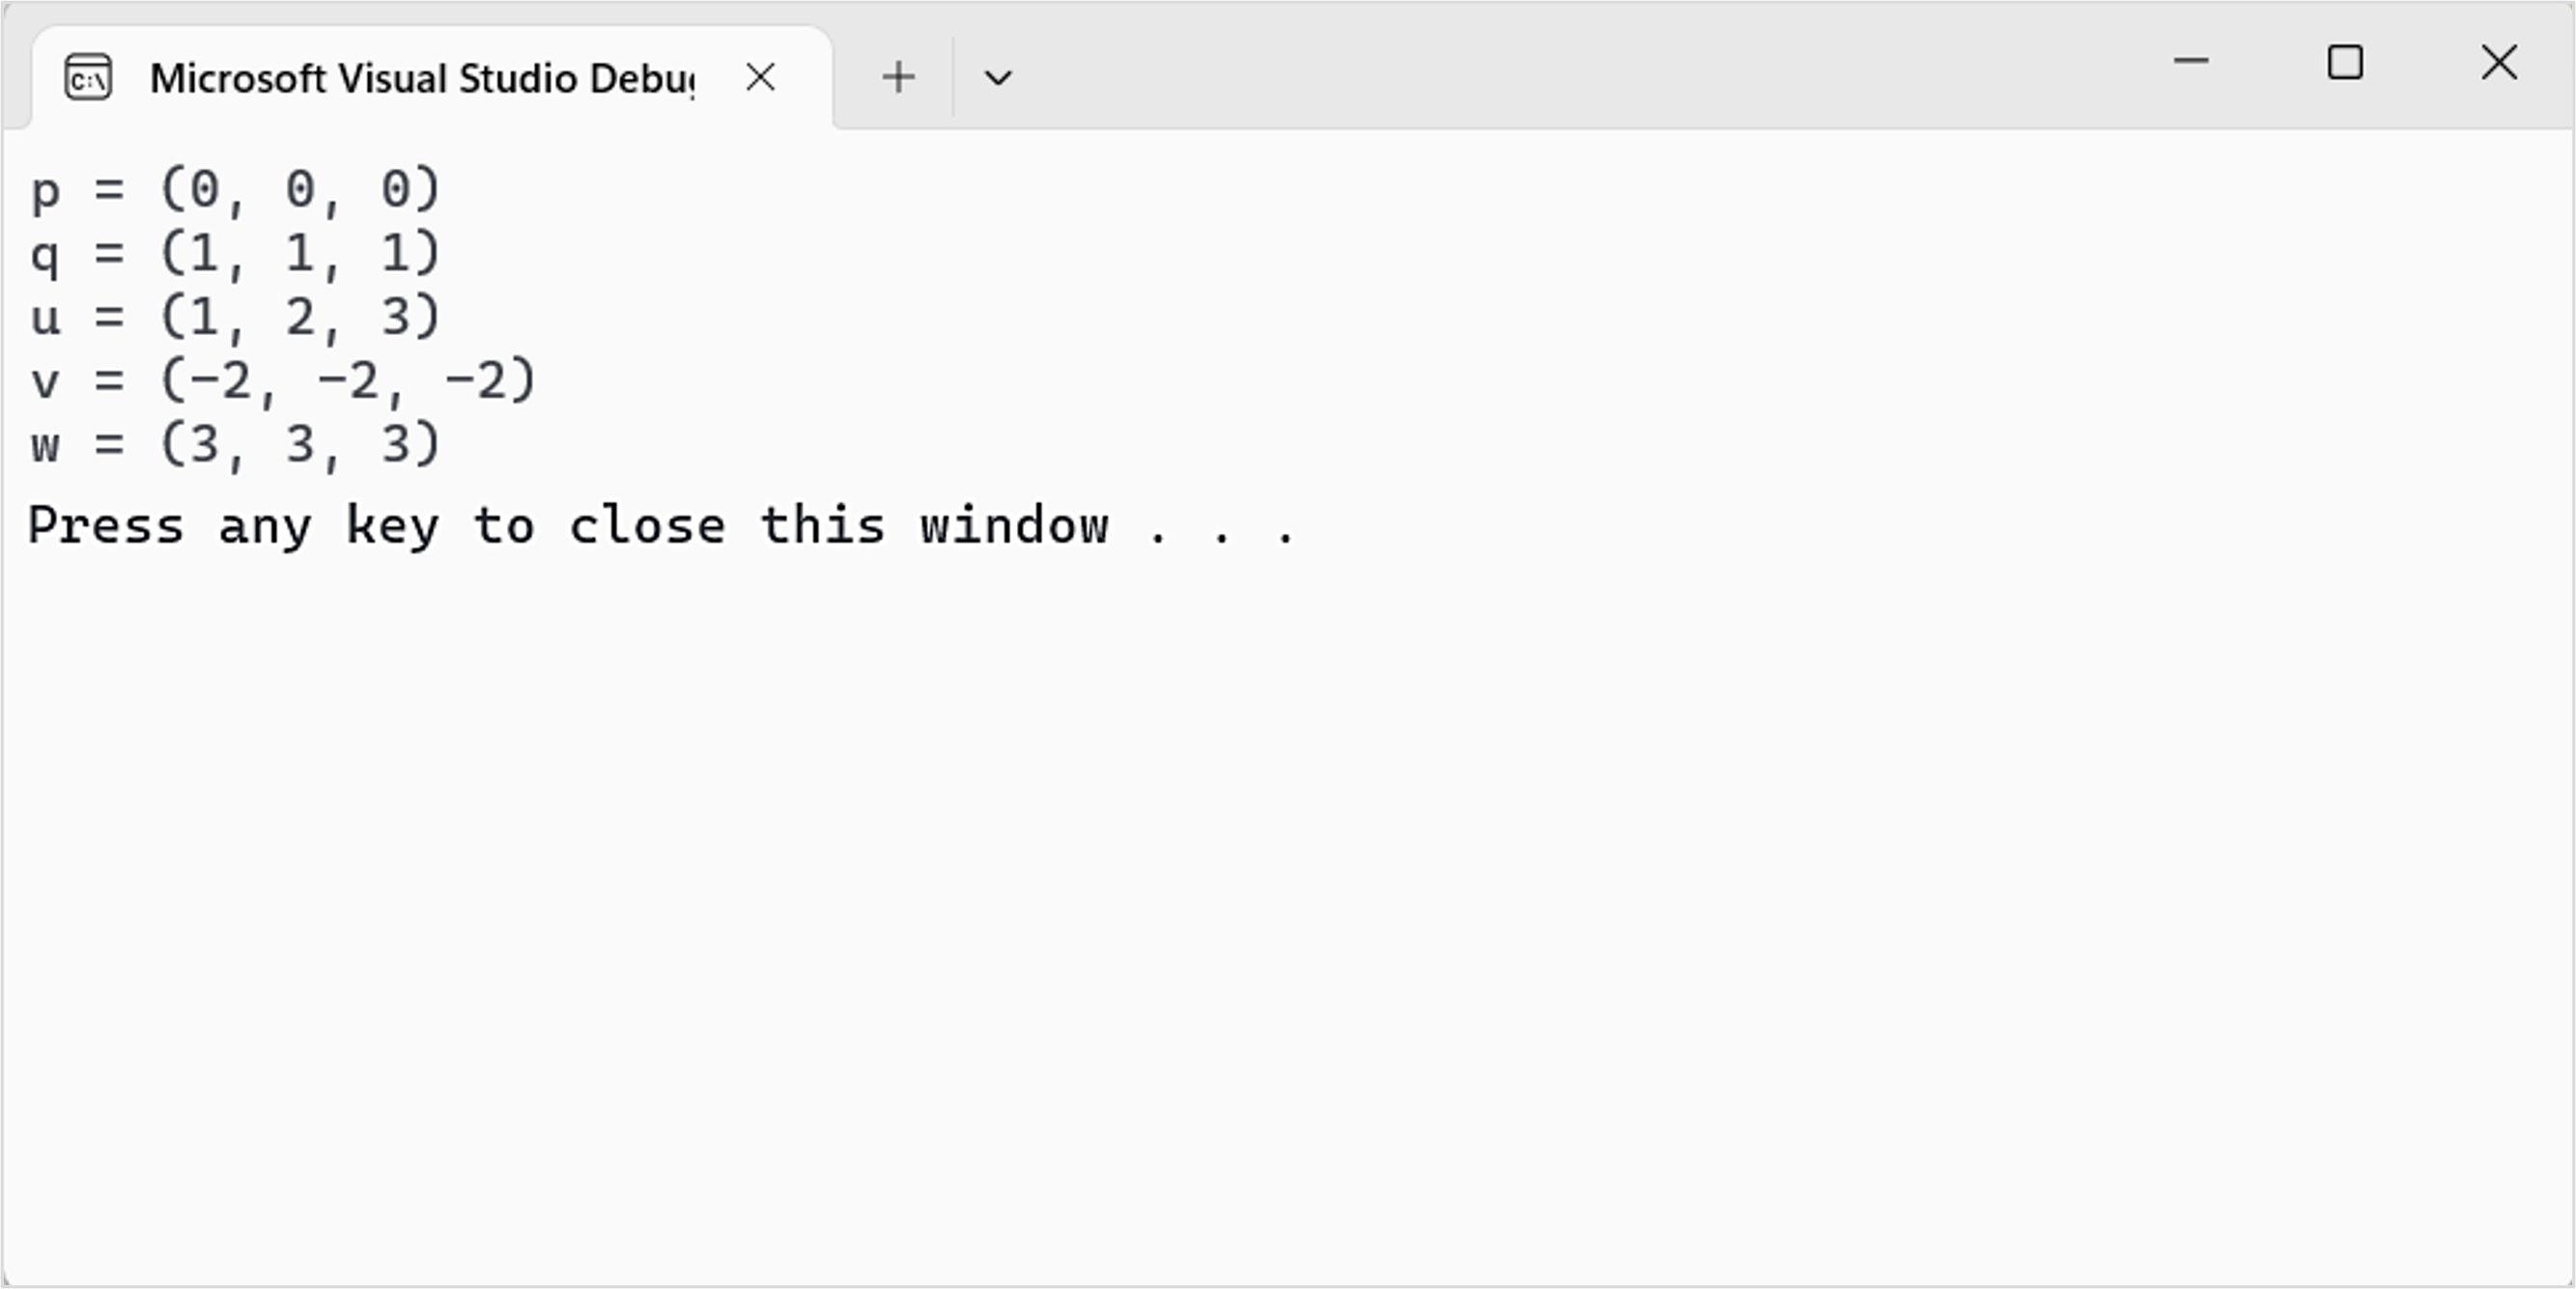
\includegraphics[width=0.8\textwidth]{Images/4/4.Session.1.1.18}
            \caption {خروجی برنامه ی بالا.}
            \label{fig:4.Session.1.1.18}
        \end{figure}
    \end{spacing}
}

\textbf{\vspace{-10pt}}
\subsection{\textbf{توابع بردار}}
{
    \Large
    \begin{spacing}{1.5}
        \lr{DirectX Math} توابع زیر را برای انجام عملیات برداری مختلف ارائه می دهد.
        ما با نسخه‌های سه‌بعدی نشان می‌دهیم، اما نسخه‌های مشابهی برای دو بعدی و چهار بعدی وجود دارد.
        نسخه های دو بعدی و چهار بعدی همان نام های نسخه های سه بعدی را دارند، به استثنای 2 و 4 که به ترتیب جایگزین 3 شده اند.
        \textbf{\vspace{6pt}}
        \lr{\lstinputlisting[language=C++,  firstline=267, lastline=304]{Codes/main.c}}
        \textbf{\vspace{-20pt}}
        \begin{point}{pnt:7}
            \Large
            توجه کنید که این توابع حتی برای عملیاتی که از نظر ریاضی یک اسکالر را برمی‌گردانند، \texttt{XMVECTOR} برمی‌گردانند (مثلاً حاصل ضرب نقطه‌ای $k=\textbf{v}_{1}\cdot\textbf{v}_{2}$).
            نتیجه اسکالر در هر جزء از \texttt{XMVECTOR} تکرار می شود. به عنوان مثال، برای حاصل ضرب نقطه، بردار برگشتی ($\textbf{v}_{1}\cdot\textbf{v}_{2},\textbf{v}_{1}\cdot\textbf{v}_{2},\textbf{v}_{1}\cdot\textbf{v}_{2},\textbf{v}_{1}\cdot\textbf{v}_{2}$) خواهد بود.
            یکی از دلایل این امر به حداقل رساندن اختلاط عملیات بردار اسکالر و \lr{SIMD} است.
            کارآمدتر است که همه چیز \lr{SIMD} را تا زمانی که محاسبات خود را تمام کنید حفظ کنید.
        \end{point}
        \textbf{\vspace{6pt}}
        برنامه ی زیر نحوه استفاده از اکثر این توابع و برخی از اپراتورهای بارگذاری شده را نشان می دهد:
        \textbf{\vspace{6pt}}
        \lr{\lstinputlisting[language=C++, caption={GITHUB/src/Chapter 1 Vector Algebra/XMVECTOR/xmvec3.cpp}, firstline=308, lastline=384]{Codes/main.c}}
        \textbf{\vspace{-30pt}}
        \begin{figure}[H]
            \centering
            \setlength{\belowcaptionskip}{-10pt}
            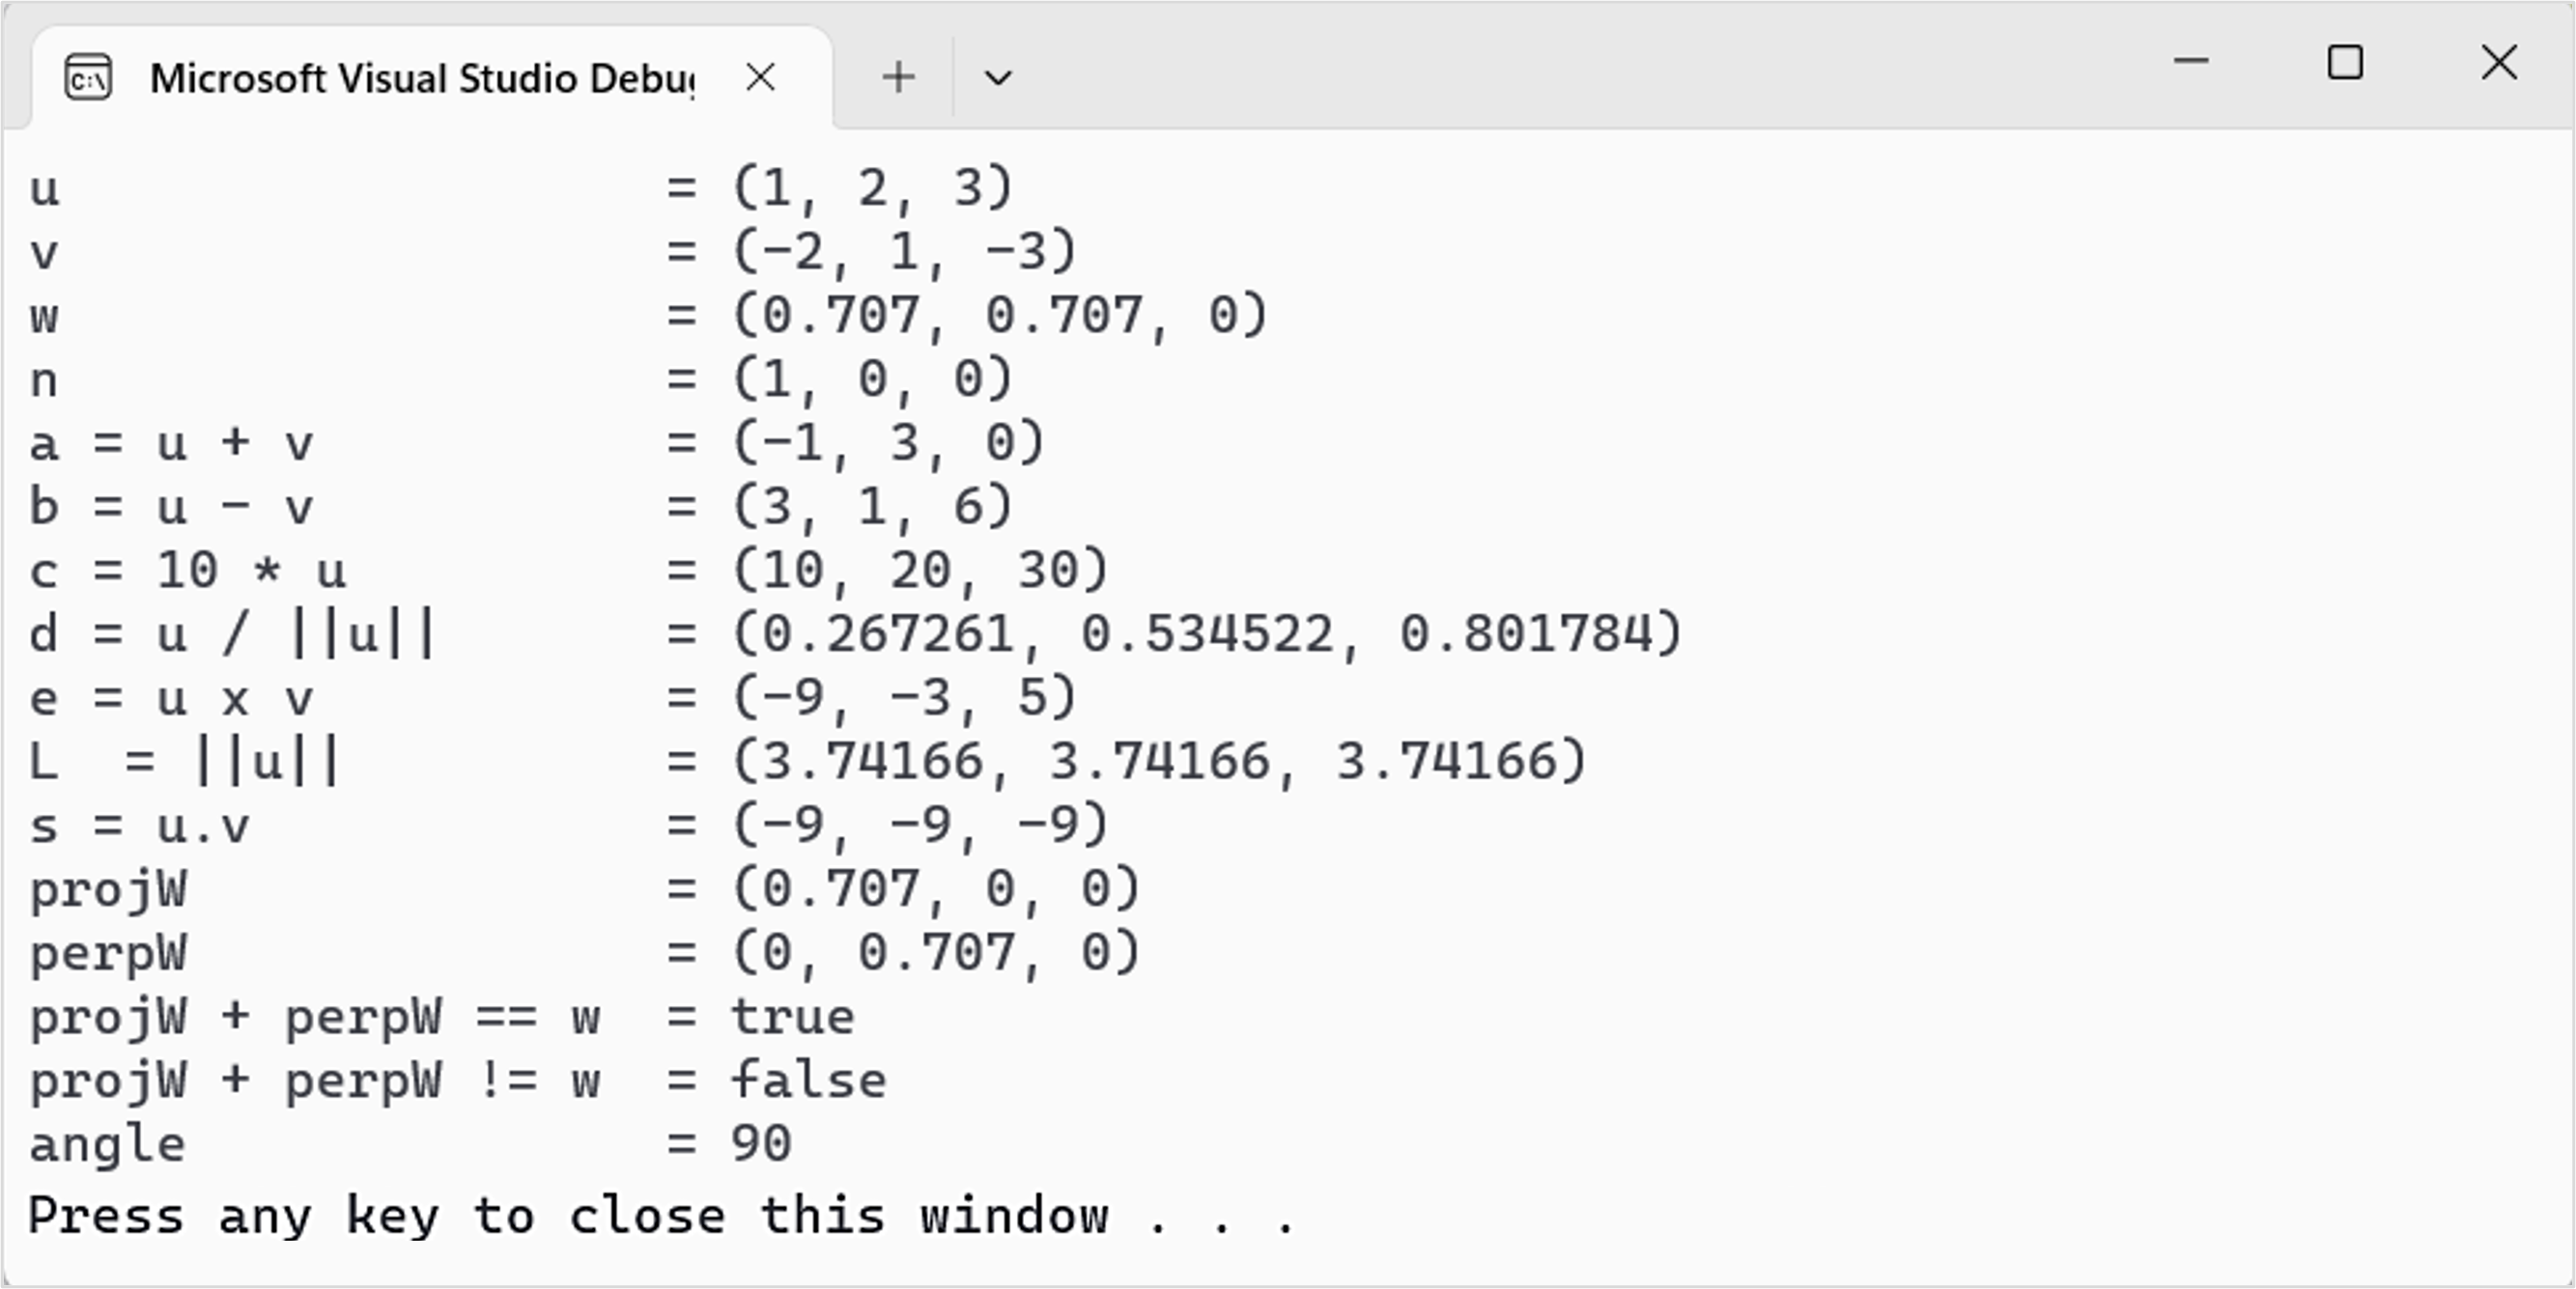
\includegraphics[width=0.8\textwidth]{Images/4/4.Session.1.1.19}
            \caption {خروجی برنامه ی بالا.}
            \label{fig:4.Session.1.1.19}
        \end{figure}
        \textbf{\vspace{-30pt}}

        \begin{point}{pnt:8}
            \Large
            کتابخانه DirectX شامل برخی از روش‌های تخمینی می‌شود که دقت کمتری دارند اما محاسبه سریع‌تر است.
            اگر مایلید کمی دقت را فدای سرعت کنید، از روش‌های برآورد استفاده کنید:
            \textbf{\vspace{6pt}}
            \lr{\lstinputlisting[language=C++,  firstline=389, lastline=392]{Codes/main.c}}
            \textbf{\vspace{-40pt}}
        \end{point}
    \end{spacing}
}

\subsection{\textbf{خطای ممیز شناور}}
{
    \Large
    \begin{spacing}{1.5}
        در مورد کار با بردارها در کامپیوتر باید به موارد زیر توجه داشته باشیم.
        هنگام مقایسه اعداد ممیز شناور، به دلیل عدم دقت ممیز شناور باید مراقب بود.
        دو عدد ممیز شناور که انتظار داریم برابر باشند ممکن است کمی متفاوت باشند.
        برای مثال، از نظر ریاضی، انتظار داریم که یک بردار نرمال شده دارای طول 1 باشد، اما در یک برنامه کامپیوتری، طول آن تقریباً $1$ خواهد بود.
        علاوه بر این، از نظر ریاضی، $1^p=1$ برای هر عدد واقعی $p$، اما زمانی که ما فقط یک تقریب عددی برای $1$ داشته باشید، می بینیم که تقریب افزایش یافته به توان $p$ ام باعث افزایش خطا می شود.
        بنابراین، خطای عددی نیز جمع می شود. برنامه کوتاه زیر این ایده ها را نشان می دهد:
        \textbf{\vspace{6pt}}
        \lr{\lstinputlisting[language=C++, caption={GITHUB/src/Chapter 1 Vector Algebra/XMVECTOR/tol.cpp}, firstline=396, lastline=428]{Codes/main.c}}
        \textbf{\vspace{-30pt}}
        \begin{figure}[H]
            \centering
            \setlength{\belowcaptionskip}{-10pt}
            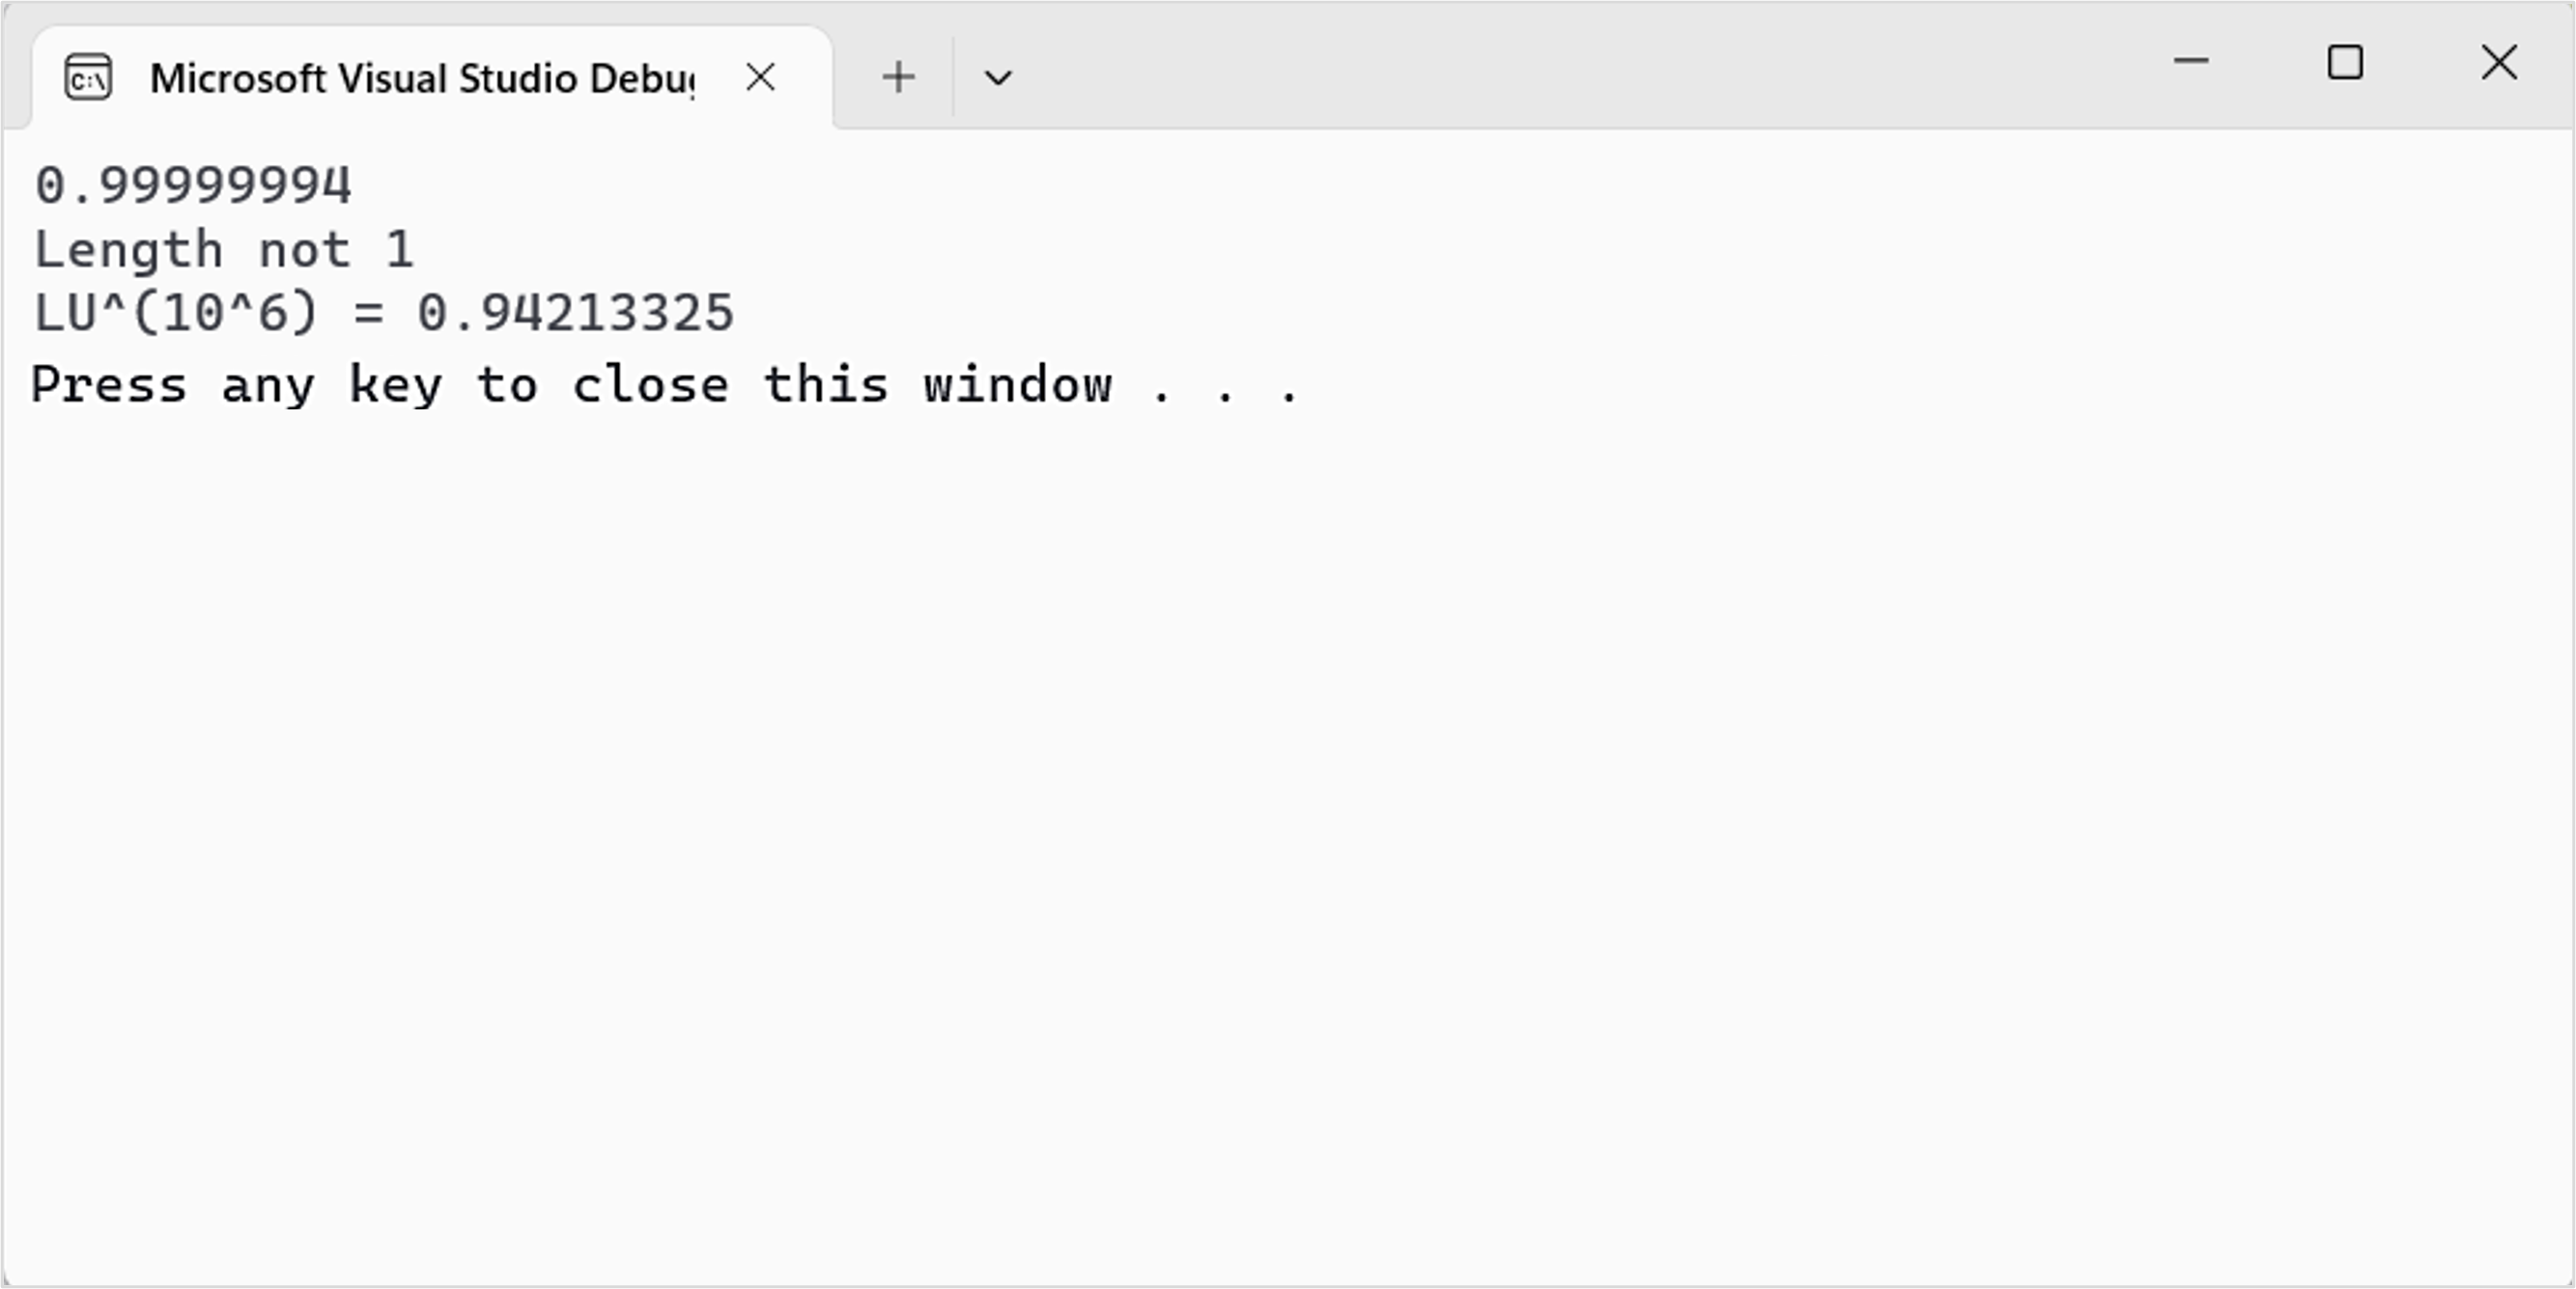
\includegraphics[width=0.8\textwidth]{Images/4/4.Session.1.1.20}
            \caption {خروجی برنامه ی بالا.}
            \label{fig:4.Session.1.1.20}
        \end{figure}

        برای جبران عدم دقت نقطه فلور، آزمایش می کنیم که آیا دو عدد نقطه فلور تقریباً برابر هستند یا خیر
        ما این کار را با تعریف یک ثابت اپسیلون انجام می دهیم، که مقدار بسیار کوچکی است که ما به عنوان بافر استفاده می کنیم.
        می گوییم دو مقدار تقریباً برابر هستند اگر فاصله آنها از اپسیلون کمتر باشد.
        به عبارت دیگر، اپسیلون مقداری تحمل برای \lr{fl} به ما می دهد.
        عملکرد زیر نشان می دهد که چگونه می توان از اپسیلون برای آزمایش مساوی بودن دو مقدار نقطه فلور استفاده کرد:
        \textbf{\vspace{6pt}}
        \lr{\lstinputlisting[language=C++,  firstline=432, lastline=436]{Codes/main.c}}
        \textbf{\vspace{6pt}}
        کتابخانه ریاضی \lr{DirectX} تابع \lr{XMVector3NearEqual} را هنگام آزمایش برابری بردارها با پارامتر اپسیلون تحمل مجاز ارائه می دهد:
        \textbf{\vspace{6pt}}
        \lr{\lstinputlisting[language=C++,  firstline=440, lastline=447]{Codes/main.c}}
    \end{spacing}
}

\textbf{\vspace{-65pt}}
\section{\textbf{خلاصه}}
{
    \Large
    \begin{spacing}{1.5}
        \begin{enumerate}
            \item {بردارها برای مدل‌سازی کمیت‌های فیزیکی استفاده می‌شوند که هم قدر و هم جهت دارند.
            از نظر هندسی، بردار را با یک پاره خط جهت نشان می دهیم.
            زمانی که یک بردار به موازات خودش ترجمه شود به طوری که دنباله آن با مبدأ سیستم مختصات منطبق باشد در موقعیت استاندارد قرار دارد.
            یک بردار در موقعیت استاندارد را می توان با تعیین مختصات سر آن نسبت به یک سیستم مختصات به صورت عددی توصیف کرد.}
            \\
            \item {اگر $\textbf{u}=(u_{x},u_{y},u_{z})$ و  $\textbf{v}=(v_{x},v_{y},v_{z})$ باشد، عملیات های برداری زیر را داریم:}

            \begin{itemize}
                \item {جمع: $\textbf{u}+\textbf{v}=(u_{x}+v_{x},u_{y}+v_{y},u_{z}+v_{z})$}
                \item {تفریق: $\textbf{u}-\textbf{v}=(u_{x}-v_{x},u_{y}-v_{y},u_{z}-v_{z})$}
                \item {ضرب اسکالر: $k\textbf{u}=(ku_{x},ku_{y},ku_{z})$}
                \item {طول: $\norm{\textbf{u}}=\sqrt{\displaystyle x^2+y^2+z^2}$}
                \item {نرمال کردن: $\hat{\textbf{u}}=\frac{\displaystyle\textbf{u}}{\displaystyle\norm{\textbf{u}}}=\left(\frac{\displaystyle x}{\displaystyle\norm{\textbf{u}}},
                \frac{\displaystyle y}{\displaystyle\norm{\textbf{u}}}, \frac{\displaystyle z}{\displaystyle\norm{\textbf{u}}}\right)$}
                \item {ضرب داخلی: $\textbf{u}\cdot\textbf{v}=u_{x}v_{x}+u_{y}v_{y}+u_{z}v_{z}$}
                \item {ضرب خارجی: $\textbf{w}=\textbf{u}\times\textbf{v}=(u_{y}v_{z}-u_{z}v_{y}, u_{z}v_{x}-u_{x}v_{z}, u_{x}v_{y}-u_{y}v_{z})$}
                \textbf{\vspace{20pt}}
            \end{itemize}

            \item {ما از نوع \lr{DirectX Math XMVECTOR} برای توصیف موثر بردارها در کد با استفاده از عملیات \lr{SIMD} استفاده می کنیم.
            برای اعضای داده کلاس، از کلاس‌های \texttt{XMFLOAT2}، \texttt{XMFLOAT3} و \texttt{XMFLOAT4} استفاده می‌کنیم و
            سپس از روش‌های بارگذاری و ذخیره‌سازی برای تبدیل بین \texttt{XMVECTOR} و \texttt{XMFLOATn} به عقب و جلو استفاده می‌کنیم.
            بردارهای ثابتی که به نحو اولیه نیاز دارند باید از نوع \texttt{XMVECTORF32} استفاده کنند.}
            \\
            \item {برای اهداف کارایی، مقادیر \texttt{XMVECTOR} را می توان به عنوان آرگومان به توابع در ثبات های \lr{SSE/SSE2} به جای روی پشته ارسال کرد.
            برای انجام این کار به صورت مستقل از پلتفرم، از انواع \texttt{FXMVECTOR}، \texttt{GXMVECTOR}، \texttt{HXMVECTOR} و \texttt{CXMVECTOR} برای عبور پارامترهای \texttt{XMVECTOR} استفاده می کنیم.
            سپس قانون عبور پارامترهای \texttt{XMVECTOR} این است که سه پارامتر اول \texttt{XMVECTOR} باید از نوع \texttt{FXMVECTOR} باشند. \texttt{XMVECTOR} چهارم باید از نوع \texttt{GXMVECTOR} باشد.
            پنجمین و ششمین پارامتر \texttt{XMVECTOR} باید از نوع \texttt{HXMVECTOR} باشد. و هر پارامتر اضافی \texttt{XMVECTOR} باید از نوع \texttt{CXMVECTOR} باشد.}
            \\
            \item {کلاس \texttt{XMVECTOR} عملگرهای حسابی را برای انجام جمع برداری، تفریق و ضرب اسکالر بارگذاری می کند.
            علاوه بر این، کتابخانه ریاضی \lr{DirectX} توابع مفید زیر را برای محاسبه طول یک بردار، مجذور طول یک بردار، محاسبه حاصل ضرب نقطه‌ای دو بردار، محاسبه حاصل ضرب متقاطع دو بردار و نرمال کردن یک بردار ارائه می‌کند:
            \textbf{\vspace{6pt}}
            \lr{\lstinputlisting[language=C++, firstline=451, lastline=455]{Codes/main.c}}
            }
        \end{enumerate}
    \end{spacing}
}

\textbf{\vspace{20pt}}
\section{\textbf{تمارین}}
{
    \Large
    \begin{spacing}{1.5}
        \begin{enumerate}
            \item {فرض کنید $\textbf{u}=(1,2)$ و $\textbf{v}=(3,-4)$. محاسبات زیر را انجام دهید و محاسبات زیر را انجام دهید و بردارها را نسبت به یک سیستم مختصات دو بعدی رسم کنید.}
            \begin{flushleft}
                \lr{
                        {(a) $\textbf{u}+\textbf{v}$} \\
                    {(b) $\textbf{u}-\textbf{v}$} \\
                    {(c) $2\textbf{u}+\frac{\displaystyle 1}{\displaystyle 2}\textbf{v}$} \\
                    {(d) $-2\textbf{u}+\textbf{v}$}
                }
            \end{flushleft}
            \\
            \item {فرض کنید $\textbf{u}=(-1,3,2)$ و $\textbf{v}=(3,-4,1)$. محاسبات زیر را انجام دهید.}
            \begin{flushleft}
                \lr{
                        {(a) $\textbf{u}+\textbf{v}$} \\
                    {(b) $\textbf{u}-\textbf{v}$} \\
                    {(c) $3\textbf{u}+2\textbf{v}$} \\
                    {(d) $-2\textbf{u}+\textbf{v}$}
                }
            \end{flushleft}
            \\
            \item {این تمرین نشان می‌دهد که جبر برداری در بسیاری از ویژگی‌های خوب اعداد حقیقی مشترک است (این فهرست جامعی نیست).
                $\textbf{u}=(u_{x},u_{y},u_{z})$، $\textbf{v}=(v_{x},v_{y},v_{z})$ و $\textbf{w}=(w_{x},w_{y},w_{z})$ را فرض کنید. همچنین فرض کنید که $c$ و $k$ اسکالر هستند. خواص برداری زیر را ثابت کنید.}
            \begin{flushleft}
                \lr{
                        {(a) $\textbf{u}+\textbf{v}=\textbf{v}+\textbf{u}$} \\
                    {(b) $\textbf{u}+(\textbf{v}+\textbf{w})=(\textbf{u}+\textbf{v})+\textbf{w}$} \\
                    {(c) $(ck)\textbf{u}=c(k\textbf{u})$} \\
                    {(d) $k(\textbf{u}+\textbf{v})=k\textbf{u}+k\textbf{v}$}
                    {(e) $\textbf{u}(k+c)=k\textbf{u}+c\textbf{u}$}
                }
            \end{flushleft}
            \begin{hint}{hnt:1}
                \Large
                فقط از تعریف عملیات برداری و خصوصیات اعداد حقیقی استفاده کنید.
                به عنوان مثال،
                \begin{equation*}
                    \centering
                    \begin{split}
                    (ck)
                        \textbf{u}&=(ck)(u_x,u_y,u_z)\\
                        &=((ck)u_x,(ck)u_y,(ck)u_z)\\
                        &=(c(ku_x),c(ku_y),c(ku_z))\\
                        &=c(ku_x,ku_y,ku_z)\\
                        &=c(k\textbf{u})
                    \end{split}
                \end{equation*}
            \end{hint}
            \\
            \item {معادله ی $2((1,2,3)-\textbf{x}=-(-2,0,4)=-2(1,2,3)$ را برای $x$ حل کنید.}
            \\
            \item {فرض کنید $\textbf{u}=(-1,3,2)$ و $\textbf{v}=(3,-4,1)$. و را نرمال کنید.}
            \\
            \item {فرض کنید $k$ یک اسکالر باشد و $\textbf{u}=(u_x,u_y,u_z)$. ثابت کنید $\norm{k}\textbf{u}=\abs{k}\norm{\textbf{u}}$. }
            \\
            \item {زاویه بین \textbf{u} و \textbf{v} متعامد(قائم)، تند یا منفرجه(باز) است؟}
            \begin{flushleft}
                \lr{
                        {(a) $\textbf{u}=(1,1,1), \textbf{v}=(2,3,4)$} \\
                    {(b) $\textbf{u}=(1,1,0), \textbf{v}=(-2,2,0)$} \\
                    {(c) $\textbf{u}=(-1,-1,-1), \textbf{v}=(3,1,0)$}
                }
            \end{flushleft}
            \\
            \item {فرض کنید $\textbf{u}=(-1,3,2)$ و $\textbf{v}=(3,-4,1)$. زاویه $\theta$ بین $\textbf{u}$ و $\textbf{v}$ را پیدا کنید.}
            \\
            \item {فرض کنید $\textbf{u}=(u_{x},u_{y},u_{z})$، $\textbf{v}=(v_{x},v_{y},v_{z})$ و $\textbf{w}=(w_{x},w_{y},w_{z})$. همچنین c و k اسکالر باشند. ویژگی های ضرب داخلی زیر را ثابت کنید.}
            \begin{flushleft}
                \lr{
                        {(a) $\textbf{u}\cdot\textbf{v}=\textbf{v}\cdot\textbf{u}$} \\
                    {(b) $\textbf{u}\cdot(\textbf{v}+\textbf{w})=\textbf{u}\cdot\textbf{v}+\textbf{u}\cdot\textbf{w}$} \\
                    {(c) $k(\textbf{u}\cdot\textbf{v})=(k\textbf{u})\cdot\textbf{v}=\textbf{u}\cdot(k\textbf{v})$}
                    {(d) $\textbf{v}\cdot\textbf{v}=\norm{\textbf{v}}^2$}
                    {(e) $\textbf{0}\cdot\textbf{v}=0$}
                }
            \end{flushleft}
            \begin{hint}{hnt:2}
                \Large
                فقط از تعاریف استفاده کنید، برای مثال،
                \begin{equation*}
                    \centering
                    \begin{split}
                        \textbf{v}\cdot\textbf{v}&=v_{x}v_{x}+v_{y}v_{y}+v_{z}v_{z}) \\
                        &=v_{x}^2+v_{y}^2+v_{z}^2 \\
                        &=\left( \sqrt{\displaystyle v_{x}^2+v_{y}^2+v_{z}^2} \right) \\
                        &=\norm{\textbf{v}}^2
                    \end{split}
                \end{equation*}
            \end{hint}
            \\
            \item {از قانون کسینوس ($c^2=a^2+b^2-2ab\cos\theta$) برای نشان دادن معادله ی زیر استفاده کنید که در آن a، b و c طول اضلاع یک مثلث و  زاویه بین ضلع های a و b است.}
            \begin{center}
                $u_{x}v_{x}+u_{y}v_{y}+u_{z}v_{z}=\norm{\textbf{u}}\norm{\textbf{v}}\cos\theta$
            \end{center}
            \begin{hint}{hnt:3}
                \Large
                شکل \ref{fig:4.Session.1.1.9} را در نظر بگیرید و $c^2=\norm{\textbf{u}-\textbf{v}}$، $a^2=\norm{\textbf{u}}$ و $b^2=\norm{\textbf{v}}$ را فرض کرده و از ویژگی های ضرب داخلی تمرین قبلی استفاده کنید.
            \end{hint}
            \\
            \item {فرض کنید $\textbf{n}=(-1,2)$. بردار $\textbf{g}=(0,-9.8)$ را به مجموع دو بردار متعامد، یکی موازی با $\textbf{n}$ و دیگری متعامد با $\textbf{n}$، تجزیه کنید. همچنین بردارها را نسبت به یک سیستم مختصات دوبعدی رسم کنید.}
            \\
            \item {فرض کنید $\textbf{u}=(-2,1,4)$ و $\textbf{v}=(3,-4,1)$. $\textbf{w}=\textbf{u}\times\textbf{v}$ را پیدا کنید و $\textbf{w}\cdot\textbf{u}=0$ و $\textbf{w}\cdot\textbf{v}=0$ را نشان دهید.}
            \\
            \item {فرض کنید نقاط زیر یک مثلث را نسبت به برخی از سیستم مختصات تعریف میکنند:
                $\textbf{A}=(0,0,0)$، $\textbf{B}=(0,1,3)$، و $\textbf{C}=(5,1,0)$. بردار متعامد این مثلث را پیدا کنید.}
            \begin{hint}{hnt:4}
                \Large
                دو بردار در دو یال مثلث پیدا کنید و از ضرب خارجی استفاده کنید.
            \end{hint}
            \\
            \item {ثابت کنید $\norm{\textbf{u}\times\textbf{v}}=\norm{\textbf{u}}\norm{\textbf{v}}\sin\theta$}
            \begin{hint}{hnt:5}
                \Large
                با $\norm{\textbf{u}}\norm{\textbf{v}}\abs{\sin\theta}$ شروع کنید و از اتحاد مثلثاتی $\cos^2\theta+\sin^2\theta=1\Longrightarrow\sin\theta=\sqrt{\displaystyle 1-\cos^2\theta}$ استفاده کنید. سپس معادله ی \ref{eqtn:4} را اعمال کنید.
            \end{hint}
            \\
            \item {ثابت کنید \norm{\textbf{u}\times\textbf{v}} مساحت متوازی الاضلاع که توسط $\textbf{u}$ و $\textbf{v}$ پوشانده شده است را نشان می دهد. شکل \ref{fig:4.Session.1.1.21} را ببینید.}
            \begin{figure}[H]
                \centering
                \setlength{\belowcaptionskip}{-10pt}
                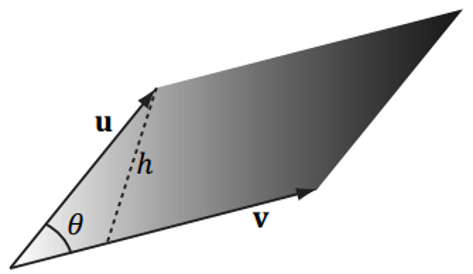
\includegraphics[width=0.5\textwidth]{Images/4/4.Session.1.1.21}
                \caption {متوازی الاضلاع توسط دو بردار سه بعدی $\textbf{u}$ و $\textbf{v}$. متوازی الاضلاع دارای پایه $\norm{\textbf{v}}$ و ارتفاع $\textbf{h}$ است.}
                \label{fig:4.Session.1.1.21}
            \end{figure}
            \\
            \item {مثالی از بردارهای سه بعدی $\textbf{u}$، $\textbf{v}$ و $\textbf{w}$ را به گونه ای بیاورید که $\textbf{u}\times(\textbf{v}\times\textbf{w})\neq(\textbf{u}\times\textbf{v})\times\textbf{w}$. این نشان می دهد که ضرب خارجی خاصیت شرکت پذیری ندارد.}
            \begin{hint}{hnt:6}
                \Large
                ترکیبی از بردارهای ساده $\textbf{i}=(1,0,0)$، $\textbf{j}=(0,1,0)$ و $\textbf{k}=(0,0,1)$ را در نظر بگیرید.
            \end{hint}
            \\
            \item {ثابت کنید که ضرب خارجی دو بردار موازی غیر صفر، بردار صفر است. یعنی $\textbf{u}\timesk\textbf{u}=0$.}
            \begin{hint}{hnt:7}
                \Large
                فقط از تعریف ضرب خارجی استفاده کنید.
            \end{hint}
            \\
            \item {مجموعه بردارهای $\{(1, 0, 0), (1, 5, 0), (2, 1, -4)\}$ را با استفاده از فرآیند گرام اشمیت، متعارف کنید.}
            \\
            \item {برنامه و خروجی زیر را در نظر بگیرید.
            تخمین بزنید که هر تابع \texttt{XMVector*} چه می کند. سپس هر تابع را در مستندات \lr{DirectXMath} جستجو کنید.}
            \textbf{\vspace{6pt}}
            \lr{\lstinputlisting[language=C++, caption={GITHUB/src/Chapter 1 Vector Algebra/XMVECTOR/VectorOps.cpp}, firstline=459, lastline=506]{Codes/main.c}}
            \textbf{\vspace{-30pt}}
            \begin{figure}[H]
                \centering
                \setlength{\belowcaptionskip}{-10pt}
                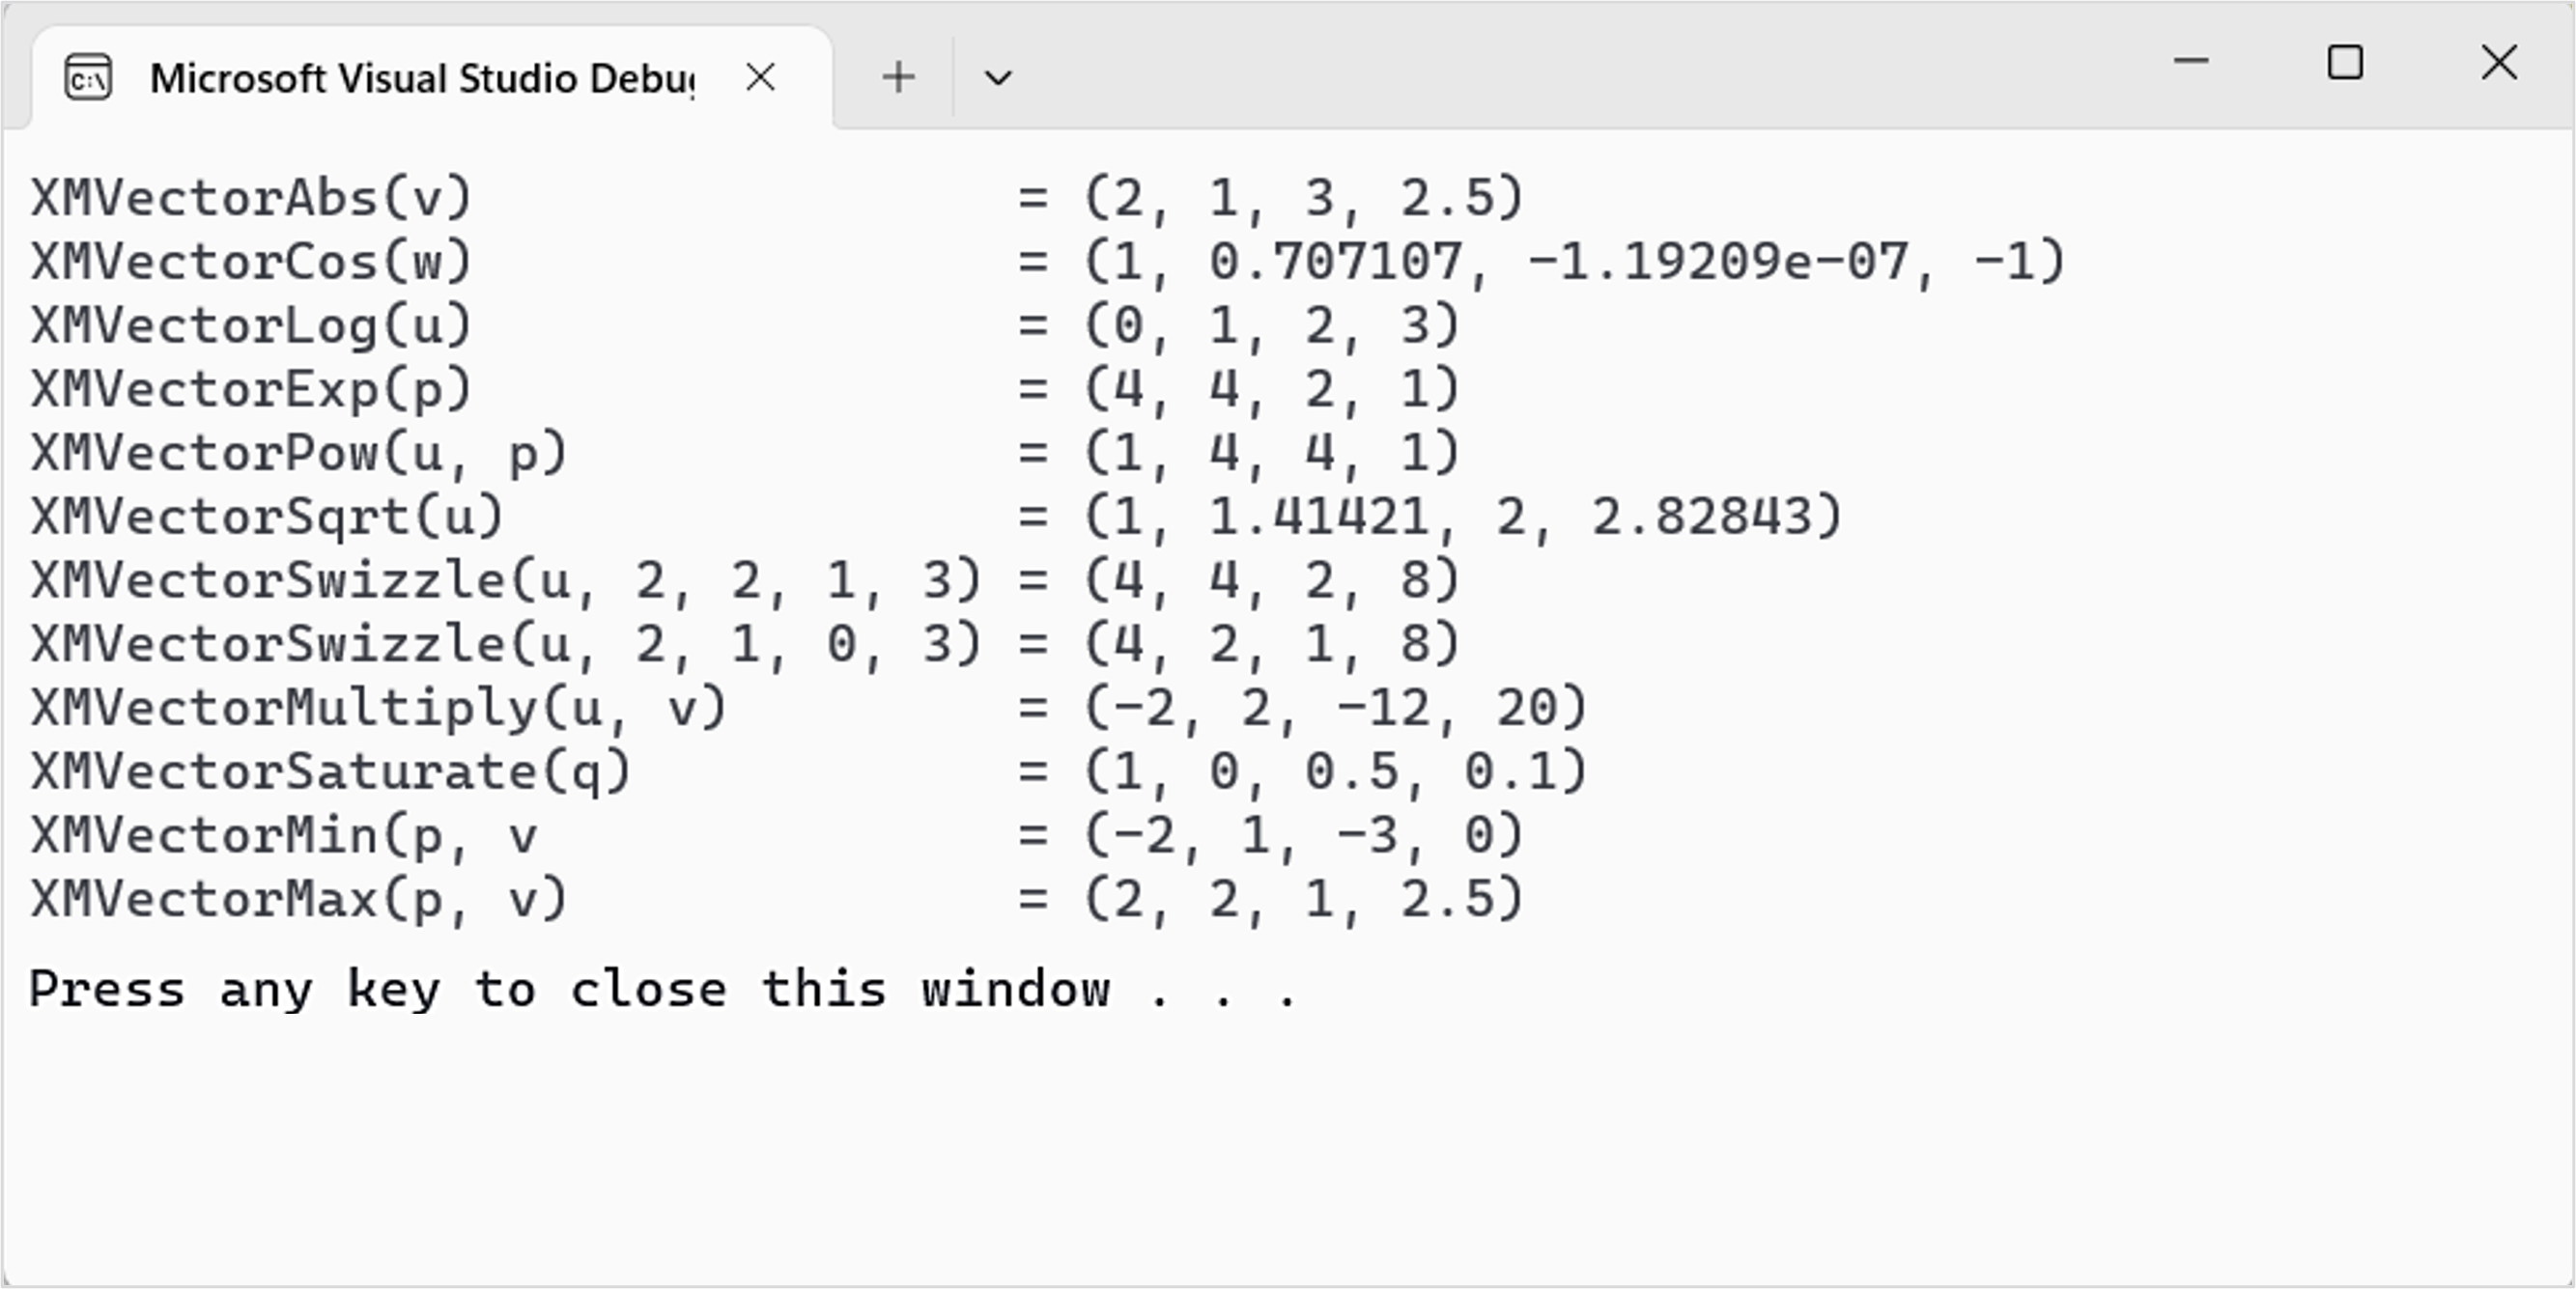
\includegraphics[width=0.8\textwidth]{Images/4/4.Session.1.1.22}
                \caption {خروجی برنامه ی بالا.}
                \label{fig:4.Session.1.1.22}
            \end{figure}
        \end{enumerate}
    \end{spacing}
}